\documentclass[english, 12pt, a4paper, elec, utf8, a-2b, online]{aaltothesis}

%% DO NOT MOVE OR REMOVE \setupthesisfonts
\setupthesisfonts

%%
%% Add here the packges you need
%%
\usepackage{graphicx}
\usepackage{algorithm}
\usepackage{algpseudocode}
\usepackage{amsmath}
\usepackage{amsfonts}
\usepackage{subcaption}
\usepackage{cleveref}
\usepackage[most]{tcolorbox} % loads tcolorbox with many default libraries


%% For tables that span multiple pages; used to split a paraphrasing example in
%% the appendix. If you don't need it, remove it.
\usepackage{longtable}

%% A package for generating Creative Commons copyright terms. If you don't use
%% the CC copyright terms, remove it, since otherwise undesired information may
%% be added to this document's metadata.
\usepackage[type={CC}, modifier={by-nc-sa}, version={4.0}]{doclicense}
%% Find below three examples for typesetting the CC license notice.


%% Edit to conform to your degree programme
%% Capitalise the words in the name of the degree programme: it's a name
\degreeprogram{Computer, Communication and Information Sciences}
%%

%% Your major
%%
\major{Algorithms}
%%

%% Choose one of the three below
%%
%\univdegree{BSc}
\univdegree{MSc}
%\univdegree{Lic}
%%

%% Your name (self explanatory...)
%%
\thesisauthor{Tianxing Wu}
%%

%% Your thesis title and possible subtitle comes here and possibly, again,
%% together with the Finnish or Swedish abstract. Do not hyphenate the title
%% (and subtitle), and avoid writing too long a title. Should LaTeX typeset a
%% long title (and/or subtitle) unsatisfactorily, you might have to force a
%% linebreak using the \\ control characters. In this case...
%% * Remember, the title should not be hyphenated!
%% * A possible 'and' in the title should not be the last word in the line; it
%%   begins the next line.
%% * Specify the title (and/or subtitle) again without the linebreak characters
%%   in the optional argument in box brackets. This is done because the title
%%   is part of the metadata in the pdf/a file, and the metadata cannot contain
%%   linebreaks.
%%
\thesistitle{MPC in practice}
\thesissubtitle{MPC in practice}
\place{Espoo}
\date{10 July 2024}

\supervisor{Prof.\ Jukka Suomela}
%%

%% Advisor(s)---two at the most---of the thesis. Check with your supervisor how
%% many official advisors you can have.
%%
\advisor{Hossein Vahidi}
%%

%% Aaltologo: syntax:
%% \uselogo{?|!|''}
%% The logo language is set to be the same as the thesis language.
%%
%\uselogo{?}
%\uselogo{!}
\uselogo{''}

\copyrighttext{\noexpand\textcopyright\ \number\year. This work is 
	licensed under a Creative Commons "Attribution-NonCommercial-ShareAlike 4.0 
	International" (BY-NC-SA 4.0) license.}{\noindent\textcopyright\ \number
	\year \ \doclicenseThis}
%%%%%%%%%%%%%%%%%%%%%%%%%%%%%%%%%%%%%%%%%%%%%%%%%%%%%%%%%%%%%%%%%%%%%%%%%%%%%%%%
\newcommand{\mstalgo}{$MST\_\log\log{n}$}

\keywords{Distributed computing, Supercomputing, Congested clique, MST, Puhti, MPI, CUDA, MPC}

\thesisabstract{
This thesis investigates the performance of Congested Clique algorithms on modern supercomputers, specifically Puhti, a Finnish supercomputer hosted by CSC.\\
The study focuses on a representative algorithm, \mstalgo{}, which is implemented using two different programming paradigms: OpenMPI (Message Passing Interface) for CPUs and CUDA (Compute Unified Device Architecture) for GPUs. The goal is to evaluate the compatibility of modern computing architectures with the Congested Clique model.\\
The evaluation examines several aspects, including how distributed computation and communication in the Congested Clique model are translated to supercomputer architectures, the overhead introduced by this translation, and the extent to which the theoretical time complexity of the algorithm holds in practice.\\
MPI is a standardized and portable message-passing library interface widely used for parallel computing, while CUDA is a parallel computing platform and programming model developed by NVIDIA for general-purpose computing on GPUs.\\
}
% result: TODO


%% All that is printed on paper starts here
%%
\begin{document}

%% Create the coverpage
%%
\makecoverpage

\makecopyrightpage

\clearpage

\begin{abstractpage}[english]
	\abstracttext{}
\end{abstractpage}

\newpage

\dothesispagenumbering{}

\mysection{Preface}
I want to thank Professor Jukka Suomela and my advisor Hossein Vahidi for their guidance.

I also want to thank my friends for keeping me sane and alive.

\vspace{5cm}
Otaniemi, 10 July 2024\\

\vspace{5mm}
{\hfill Tianxing Wu \hspace{1cm}}

%% Force a new page after the preface
%%
\newpage


%% Table of contents. 
%%
\thesistableofcontents


%% Symbols and abbreviations
\mysection{Symbols and abbreviations}


\subsection*{Abbreviations}

\begin{tabular}{ll}
\mstalgo{}         & The algorithm described in \cite{MSTLogLogn} \\
MPI                & Message Passing Interface \\
CUDA               & Compute Unified Device Architecture \\
HPC                & High-performance computing \\
AI                 & Artificial intelligence \\
GPU                & Graphics processing unit \\
CPU                & Central processing unit \\
MST                & Minimum spanning tree \\
SLURM              & Simple Linux Utility for Resource Management \\
SM 							   & Streaming multiprocessor \\
SP 							   & Streaming processor \\
\end{tabular}

\cleardoublepage

\section{Introduction}
\label{sec:Introduction}

\thispagestyle{empty}
Congested Clique, described in \cite{powerCongestClique}, is a model for distributed computing. It features $n$ computing nodes in a clique network, sending messages in a synchronized manner. A clique network is a complete network where each computing node is connected to all other nodes. In the network, each node in the network corresponds to a node in an input graph $G$. The nodes in the network work together to solve a problem of the input graph.

The computation efficiency of the congested clique model is measured by the number of (communication) rounds it takes before the algorithm converges. In each round, each node do local computation and sends $O(\log{n})$ bits to each of its neighbor nodes. With Congested Clique, we emphasis communication over local computation in a round. Because it is believed that the communication is the bottleneck in distributed computing. We consider local computation is free, as there are unlimited computing power and memory space on each node.

We study the Congested Clique model in the context of modern distributed computing hardware, specifically supercomputers. Supercomputers are high-performance computing machines that are used for large-scale scientific and engineering problems. Unlike traditional computers, supercomputers use more than one processing unit \cite{IBMsupercomputing}. The distributed natural of supercomputers makes them a good fit for running Congested Clique algorithms.

The study is done by implementing a representative algorithm from the Congested Clique model, \mstalgo{}, on a supercomputer. The implementation is done with two different programming paradigms: OpenMPI (Message Passing Interface) for CPUs and CUDA (Compute Unified Device Architecture) for GPUs. The goal is to evaluate the compatibility of modern computing architectures with the Congested Clique model.

\subsection{Methodology}
The algorithm \mstalgo{} from \cite{MSTLogLogn} is chosen as the representative algorithm for discussion in this work. The representativeness will be later shown. It solves Minimum spanning tree ($MST$) problems in $O(\log{\log{n}})$ Congested Clique rounds. A $MST$ problem is to find a spanning tree of $G$ where its weight is as small as possible.  We show that \mstalgo{} represents the algorithms on Congested Clique so its property generalize to the whole algorithm category. 

\mstalgo{} is implemented on the supercomputer Puhti, a Finnish supercomputer hosted by CSC \cite{Puhti}. We benchmark the performance of \mstalgo{} on Puhti to study its properties. The implementation is done with two different programming schemes:
\begin{itemize}
	\item[--] Message Passing Interface ($MPI$) programming scheme with CPUs.
	\item[--] Compute Unified Device Architecture ($CUDA$) programming scheme with Nvidia GPUs.
\end{itemize}

We run \mstalgo{} with both CPUs and GPUs because they are two different types of computing hardware on modern computers. They follows different programming paradigms and have different hardware constraints. When implementing \mstalgo{}, the coding follows best practices and common sense. We optimize how the algorithm is implemented but do not change the algorithm itself.

The graphs to solve are complete graphs with $n$ vertices, meaning they have $\frac{n(n-1)}{2}$ edges. We focus on large graphs with $n$ up to $10^4$, and $10^9$ edges.

\subsection{Objective}
The purpose of this work is to identify the connections between the Congested Clique model and modern distributed computing hardware, software and tools. We demonstrate our solution to simulate congested clique algorithms with HPC hardware by making reasonable design decision in regards of:
\begin{itemize}
	\item[--] How to share data between machines.
	\item[--] How to allocate workload to machines so the hardware is utilized efficiently.
	\item[--]	How to synchronize the communication in a rounds based fashion.
\end{itemize}
We evaluate the performance of the simulation and analyze how the hardware limits the performance of the algorithm in terms of memory, CPU, GPU, and network. We try to answer what assumptions Congested Clique makes bring the performance bottleneck, and with what setting will the bottleneck appear. We also discuss with what setting the algorithm performs as Congested Clique model expects.

We compare how the \mstalgo{} performs compared to its sequential alternative, in terms of:
\begin{itemize}
	\item[--] Capability of processing large graphs, with large number of vertices and edges.
	\item[--] Wall clock time when processing the same graphs.
\end{itemize}
We discuss how is the scalability of the \mstalgo{}:
\begin{itemize}
	\item[--] Strong scaling and weak scaling (How having more processes speeds up the computation, which part of the hardware will become bottleneck when scaling continuously).
	\item[--] Time composition for the run when scaling (MPI\_time vs local). Does the time complexity hold?
\end{itemize}
\clearpage

\section{Preliminaries}
\label{sec:preliminaries}

\subsection{Congested clique (also known as CLIQUE)}
Each node in a $n$-node Congested Clique network has a unique identifier of $O(\log{n})$ bits. In each round of a Congested Clique of $n$ nodes, each node does local computation and sends at most $O(\log{n})$ bits to each of its neighbor nodes. The nodes send messages by unicast, allowing them to send a different message on each of their links in one round. The rounds are synchronized, meaning that all nodes start and finish the round at the same time. \cite{powerCongestClique}

The Congested Clique makes the assumption that each node has unlimited computing power and memory space. Thus communication time becomes the bottleneck and the running time is only measure by the number of communication rounds.
\subsection{\mstalgo{}}
\mstalgo{} is an algorithm developed by Zvi Lotker, Boaz Patt-Shamir, Elan Pavlov, and David Peleg in 2005. It solves the Minimum Spanning Tree ($MST$) problem in $O(\log{\log{n}})$ communication rounds in the Congested Clique model.

In the \mstalgo{} algorithm, the nodes of \( G \) are partitioned into disjoint clusters. For each cluster \( F \subseteq \mathcal{F} \), there exists a minimum spanning subtree \( T(F) \). The algorithm begins with each vertex \( v_i \) forming a singleton cluster, i.e., \( \mathcal{F}^0 = \{ F_1^0, \dots, F_n^0 \} \) where \( F_i^0 = \{ v_i \} \) for \( 1 \leq i \leq n \). The clusters are iteratively merged until only a single cluster remains, at which point the algorithm terminates.

The merging process operates in phases, with each phase \( k \geq 0 \) growing the cluster size quadratically. This ensures that there are at most \( O(\log \log n) \) phases. Each phase \( k \) consists of \( O(1) \) communication rounds, implying that the \mstalgo{} algorithm completes in \( O(\log \log n) \) communication rounds.


In each phase, \mstalgo{} runs following steps:
\begin{itemize}
	\item[1.] 
	\begin{itemize}
			\item[(a)] Compute the minimum-weight edge $e(v, F')$ that connects $v$ to any node in $F'$ for all clusters $F' \neq F$.
			\item[(b)] Send $e(v, F')$ to $\ell(F')$ for all clusters $F' \neq F$.
	\end{itemize}

	\item[2.] If $v = \ell(F)$, then:
	\begin{itemize}
			\item[(a)] Using the messages received from Step 1, compute the lightest edge between $F'$ and $F$ for every other cluster $F'$.
			\item[(b)] Perform (locally) Procedure \textsc{Cheap-Out}. This procedure does the following:
			\begin{itemize}
					\item Selects a set $\mathcal{A}(F)$ containing the $N$ cheapest edges that go out of $F$ to $N = |F|$ distinct clusters.
					\item Appoints for each such edge $e$ a guardian node $g(e)$ in $F$, ensuring that each node in $F$ is appointed as guardian to at most one edge.
			\end{itemize}
	\end{itemize}

	\item[3.] Let $e' \in \mathcal{A}(F)$ be the edge for which $v$ was appointed as guardian, i.e., such that $g(e') = v$. Send $e'$ to $v_0$, the node with the minimal ID in the graph.
	
	\item[4.] If $v = v_0$, then:
	\begin{itemize}
			\item[(a)] Perform (locally) Procedure \textsc{Const-Frags}. This procedure computes $E^k$, the new set of edges to add.
			\item[(b)] For each edge $e \in E^k$, send a message to $g(e)$.
	\end{itemize}

	\item[5.] If $v$ receives a message from $v_0$ that $e \in E^k$, then $v$ sends $e$ to all nodes in the graph.

	\item[6.] Each node adds all edges in $E^k$ and computes $T$.
\end{itemize}
Newer and faster algorithms for the (MST) problem have been developed in the Congested Clique model, such as the $\log^*$-round algorithm proposed by \cite{MSTLogStar} and the constant-round algorithm from \cite{MSTConstant}. However, we have chosen to use \mstalgo{} for the following reasons:
\begin{itemize}
	\item[--] \mstalgo{} is a typical Congested Clique algorithm. The properties of \mstalgo{} generalize to the whole algorithm category.
	\item[--] \mstalgo{} is simple and easy to understand. It saves time to study and implement the algorithm. So it can be implemented with different programming schemes.
	\item[--] There is no noticeable round boost compared to \cite{MSTLogStar} and \cite{MSTConstant} within the range of graph size up to millions of edges (under 4 rounds).
\end{itemize}
The representativeness of \mstalgo{}{} can be shown in the following ways:
\begin{itemize}
	\item[--] \mstalgo{} exploit the full connectivity of the graph. In each round, there is a step where each computer sends $O(\log{n})$ messages to all the other computers.
	\item[--] To comply with the $O(\log{n})$ limit when sending to a unique leader, large data is spilled to other computers before sending.
	\item[--] The algorithm needs several rounds before its convergence.
\end{itemize}

\subsection{The super-computer Puhti}
Puhti is a supercomputer managed by CSC, designed for high-performance computing (HPC) and artificial intelligence (AI) applications. It employs the Slurm workload manager \cite{Slurm} to allocate computing resources across its nodes. The CPU model is Intel Xeon Gold 6230 (Cascade Lake architecture), featuring 20 cores per processor running at 2.1 GHz and supporting AVX-512 vector instructions and VNNI instructions optimized for AI inference workloads. Each node is equipped with two Intel Xeon processors. An Intel Xeon processors has $20$ cores. With each mappable to one slurm task, a node can have at most $2 \times 20$ tasks, supported by a total of 192 GiB of memory \cite{PuhtiDoc}.

There are 484 nodes in the "M" cluster. These nodes are connected using Mellanox HDR InfiniBand, with each node linked via a 100 Gbps HDR100 connection. The network topology follows a fat-tree structure with a blocking factor of approximately 2:1, meaning there are twice more ports going down than going up \cite{PuhtiDoc} \cite{FatTrees}. 

In addition to CPU nodes, Puhti includes an AI-dedicated partition with 80 GPU nodes, achieving a peak performance of 2.7 petaflops. Each GPU node contains two Intel Xeon processors (Cascade Lake, 20 cores each at 2.1 GHz) and four Nvidia Volta V100 GPUs with 32 GB of memory each. Each node is equipped with 384 GB of main memory and 3.6 TB of local storage, configured for GPU-intensive workloads that scale across multiple nodes. The AI partition’s interconnect uses a dual-rail HDR100 network, providing 200 Gbps aggregate bandwidth with a non-blocking fat-tree topology, enabling efficient communication across nodes \cite{PuhtiDoc}.

\subsection{Message Passing Interface (MPI)}
% TODO what is a rank
Message Passing Interface (MPI) is a standardized and portable message-passing library interface, widely used for parallel computing. It allows processes running on distributed systems to communicate with each other by sending and receiving messages. MPI supports both point-to-point communication (between individual pairs of processes) and collective communication (among multiple processes), enabling efficient data sharing and synchronization.

MPI is used extensively in high-performance computing (HPC) to coordinate computation across nodes in a cluster, leveraging both shared and distributed memory architectures \cite{MPI}.

\subsection{CUDA}

CUDA (Compute Unified Device Architecture) is a parallel computing platform and programming model developed by NVIDIA for general purpose computing on GPUs. In CUDA, the CPU is referred to as the host, while the GPU is the device. CUDA programs typically consist of both host and device code. 

A kernel function is a function that runs on the device and can be executed by many threads in parallel. Each thread performs computations independently, allowing for massive parallelism on the GPU. 

Memory allocation on the device is performed using the \texttt{cudaMalloc} function, which takes a pointer and the size of memory to be allocated in bytes:
\begin{verbatim}
cudaMalloc((void **)&devicePointer, size);
\end{verbatim}

Data can be copied between the host and device using \texttt{cudaMemcpy}, which specifies the source, destination, size, and direction (host-to-device or device-to-host). For example:
\begin{verbatim}
cudaMemcpy(devicePointer, hostPointer, size, cudaMemcpyHostToDevice);
\end{verbatim}

To launch a kernel function, specify the number of threads per block and blocks per grid using the syntax \texttt{kernel<<<gridDim, blockDim>>>(args);} where \texttt{gridDim} and \texttt{blockDim} define the grid and block dimensions:
\begin{verbatim}
kernelFunction<<<numBlocks, threadsPerBlock>>>(arguments);
\end{verbatim}

This structure allows CUDA to manage memory and computation efficiently, making it suitable for high-performance computing applications.


\clearpage

% TODO mention here we are using double precision
\section{Congested clique with MPI}
\label{sec:mpi}
% why multiple cpus, why MPI, why not just one cpu, introduce MPI
The Intel Xeon Gold 6230 CPU has 40 cores. Each core can run one Slurm task. The ability to issue multiple tasks on one CPU is the basis of the simulation. The graphs to solve can be way larger than the number of tasks on one CPU, up to $10^4$ vertices. With the naive way of simulation. To address the problem, we need both multiple vertices on one MPI rank, and multiple compute nodes that communicate with MPI. \cref{alg:mst_mpi} describes the pseudo code of the \mstalgo{} implemented with MPI.
\begin{algorithm}
	\caption{\textsc{Minimum Spanning Tree} with MPI}
	\label{alg:mst_mpi}
	\textbf{Require:} Number of vertices $n$, adjacency matrix $\mathbf{A} \in \mathbb{R}^{n \times n}$.\\
	\textbf{On each rank:} Rank index $i$, number of vertices per rank $n_r$, and adjacency sub-matrix $\mathbf{A}[i \times n_r : (i + 1) \times n_r, :] \in \mathbb{R}^{n_r \times n}$.
	\begin{algorithmic}[1]
	\State $vertex\_lo \gets i \times n_r$
	\State $vertex\_hi \gets (i + 1) \times n_r$
	\State $T \gets \emptyset$
	\While{there exists $v \notin T$}
		\If{First phase}
			\For{$v = vertex\_lo$ to $vertex\_hi$}
				\State Find the minimum edge $e(v, v')$ connected to $v$
			\EndFor
			\State \texttt{MPI\_Gather} all $e(v, v')$ to rank 0
		\Else
			\Comment{Step 1}
			\For{$v = vertex\_lo$ to $vertex\_hi$}
				\State For each fragment $F' \neq F$, compute $e(v, F') \gets \min_{v' \in F'} \{ e(v, v') \}$
				\State Add $e(v, F')$ to the send buffer
			\EndFor
			\State \texttt{MPI\_Alltoall} all $e(v, F')$ to leaders $l(F')$
			\Comment{Step 2}
			\For{$v = vertex\_lo$ to $vertex\_hi$}
				\If{$v = l(F)$}
					\State For each fragment $F' \neq F$, compute $e(v, F') \gets \min_{v' \in F'} \{ e(v, v') \}$
					\State Perform \textsc{Cheap-Out} and add the edge $e$ to the send buffer
				\EndIf
			\EndFor
			\State \texttt{MPI\_Gather} all $e$ to rank 0
			\Comment{Step 4}
		\EndIf
		\If{on rank 0}
			\State Perform \textsc{Construct-Frags} and update $T$
			\State \texttt{MPI\_Broadcast} the updated $T$ to all ranks
		\EndIf
		\Comment{Steps 5 and 6}
		\State Each rank updates $T$ with the received data
	\EndWhile
	\State \textbf{Return} the spanning tree $T$
	\end{algorithmic}
\end{algorithm}


\subsection{Communication}
Each process has its dedicated memory space and computing power, which is shared between all the nodes that the process is responsible for. 
The communication is handled by OpenMPI. OpenMPI is an open-source Message-passing Interface implementation. 
Each process is responsible for a batch of vertices with continuous indices. It maintains all the edges adjacent to the vertices and their states. It sends MPI messages to other processes in representative of the vertices. 

The communication steps in each phased can be categorized into three types. In step 1 and 2, all the nodes send messages to all other nodes. In step 4, rank 0 gathers the messages from all other nodes. In step 5 and 6, rank 0 sends messages to all other nodes.
All the three categories of communication involve all the nodes in the graph. MPI collective communication functions are well suited for these types of communication. Collective communication functions are functions that involve a group of processes \cite{MPI}.
The three category of communication can be done with \texttt{MPI\_Alltoall}, \texttt{MPI\_Gather}, and \texttt{MPI\_Broadcast} respectively.

Synchronization between ranks are done typically with \texttt{MPI\_Barrier}. However, there are only collective communication in the implementation of \mstalgo{}. They are synchronous by design. They inherently ensure that all participating ranks reach the collective call before proceeding. This means that these operations implicitly act as synchronization points. \cite{MPI}

In the beginning of \mstalgo{}, each rank receives input to run the algorithm. The input includes a list of vertices the rank is responsible for and all the adjacent edges. The MPI communication in each step is done in the following way:
\begin{itemize}
	\item[--] step 1: \texttt{MPI\_Alltoall} (comm1)
	\item[--] step 2: \texttt{MPI\_Alltoall} (comm2)
	\item[--] step 3: \texttt{MPI\_Gather} (comm3)
	\item[--] step 4: Local computation on rank 0
	\item[--] step 5: \texttt{MPI\_Broadcast} (comm4)
	\item[--] step 6: Local computation on each thread
\end{itemize}

In step 3, clusters leaders scatter messages to the guardians before the guardians forward the messages to rank 0. This step is skipped in our implementation, instead, there is a simple gather operation on rank 0 to get edges from leaders. This is because OpenMPI does optimization under the hood by using a tree-based gathering pattern \cite{MPICollective} \cite{OpenMPIRepoGather}, which is what step 3 tries to achieve. Hence, how we allocate the nodes to the ranks and the network topology affects the way to balance the traffic, it is wiser to let MPI handle the optimization.

\subsection{Simplification on the first phase}
We implement the algorithm with the best practices and common sense. The algorithm is modified to align with the implementation goal. 

At the beginning of the first phase, there is no spanning tree or clusters formed yet. Each vertex itself is a cluster. In the first step, for each vertex $v$ and edge $e \in E_v$, $e$ is sent over the connection $e$. 
Because for every two clusters $F \neq F'$, there is only one unique edge connecting them. 
In step two, each cluster leader (the vertex itself) sorts all the edges it receives, which is all the edges the vertex is adjacent to check the minimum, sort and take only one as $\mu$ is $1$. 

Essentially, all the above steps find each vertex the minimum weight edge adjacent. Simplification is done to the algorithm during the first phase. In the simplified version, rank 0 gathers the minimum weighed edges adjacent to each vertex (comm0) and skips steps 1-3 during the first phase. 

The Simplification has a significant impact on the performance of the algorithm. Because the time taken by MPI communication corresponds to the message size. During the first phase, each vertex is a cluster, and the communication needs are the biggest in the whole algorithm. 

% \subsection{Scattering to the guardians}
% In the third step, each cluster leader sends the minimum weight edge to the guardians of the cluster. before every guardian forwards the edge to rank 0. This avoids breaking the bandwidth limit if each cluster leader sends the edge to rank 0 directly in the Congest Clique. 

% However, each cluster leader forwards the edges directly to the rank 0 in our implementation. It is shown that it's more efficient. 

\subsection{Union-find}
When merging edges to the MST, each edge is checked if its addition to the tree creates a cycle. We use the union-find algorithm to do the checks efficiently. If two vertices have the same root, it means they are connected. When an edge is added to the MST, two sets containing the vertices are merged. 

\subsection{Vertex partitioning and graph generation}
Each process holds a list of vertices and all the edges adjacent to the vertices. The edges are represented in the form of adjacency matrix, which is a list of lists. Each element in the matrix is a random weight of the edge. The matrix is partitioned so that each process holds a continuous part of the matrix. 

Each node can launch at most 40 tasks with a total memory limit of 192 GiB. With $n$ task for a node, each task shares $192/n$ GiB memory. The memory size limits how many edges can be stored locally. The bottleneck comes when generating the graph. 
The naive method would be to generate the adjacency matrix entirely on rank 0. And use \texttt{MPI\_Scatter} to scatter the partitions to the destination ranks. Each rank will get a batch of matrix rows. This method is memory eager on rank 1. It needs $O(n^2)$ bits. 

Alternatively, the graph can be generated in a distributed manner, where the workload is divided among all ranks. The goal is to generate a triangular matrix with 0-diagonal, because the adjacency matrix is symmetric along the diagonal. Each rank is responsible for the part whose vertices are at. When the triangle matrix is ready, the 0's at the other side of the diagonal can be filled with \texttt{MPI\_Alltoall}.
\clearpage

\section{Performance with MPI}
\label{sec:mpi_performance}
\subsection{Conclusion overview}
% TODO the number of runs meets the expectation
When we are simulating the Congested Clique model with MPI on CPU threads, the number of threads can be utilized is limited. Partitioning the vertices to the threads is inevitable. When there are only one or a few vertices on each rank, as the Congested Clique model predicts, the communication time is the bottleneck. As we try to run larger and larger graph with limited thread resources, the communication time is no longer the majority of the total time. The thread computation time becomes the bottleneck. % fixed threads, increasing vertices case

% strong scaling case. Maybe weak scaling

% ?? We want communication time to be the majority cuz we can do optimization on the network. Better connection etc

We compare the performance of \mstalgo{} with the prim's algorithm. With the same graph, \mstalgo{} takes more compute and memory than the prim's algorithm. By increasing the number of work nodes. \mstalgo{} outperforms the prim's algorithm in terms of wall clock time. \mstalgo{} is also capable of processing larger graphs than the prim's algorithm. The bottleneck for processing larger graphs is the memory for MPI messages.

% emphasis** TODO Conclusion Simply having more tasks is not enough. but multiple v on each rank works, -> further decreases thread computation time. (memory bound for making buffer)
% we want Bigger MPI composition fraction, hardware limits (not enough threads, ideally on thread one vertex the best fraction) -> vertex partitioning
% how to do the partition better -> more ranks with less vertices on each rank (This saves the total communication time as vertices are on the same thread).
% We want better wall time -> communication time can be resolved with multiple vertices on the same rank. We want to optimize composition (The thread computation is memory bound) so more vertices can be fit on each rank (saves both communication inter nodes and better MPI communication fraction).

The number of rounds is as predicted only $O(\log{\log{n}})$. From the running time perspective, Python is significantly slower than the C++. The slowdown comes from both the MPI time and computation time. The slowdown in MPI is mainly contributed by how large space python numbers take in memory. The computation slowdown is expected as python is an interpreted language. With python, the algorithm is more memory bound. It takes much more memory to construct the MPI messages compared to the C++ counterpart.
\subsection{Performance}
We run the \mstalgo{} implementation \cref{alg:mst_mpi} with MPI on Puhti. We are benchmarking with complete graphs here. We want to learn:

\begin{itemize}
	\item[--] With limited number of thread, what is the best practice to partition the vertices.
	\item[--] How does the time composition looks like under different partitioning. Does it follow the prediction of the Congested Clique model.
	\item[--] What is the capacity - how many more edges can be processed of the algorithm, compared to a single node prim's algorithm.
	\item[--] Can the algorithm achieve better running time than the prim's algorithm processing the same graph.
\end{itemize}

We have limited thread resources, on a single computing node. Starting with 8 threads, we increase the number of vertices on each rank.

\begin{figure}[h]
	\centering
	% Top row, left (a)

	% Top row, right (b)
	\begin{subfigure}[b]{0.45\textwidth}
			\centering
			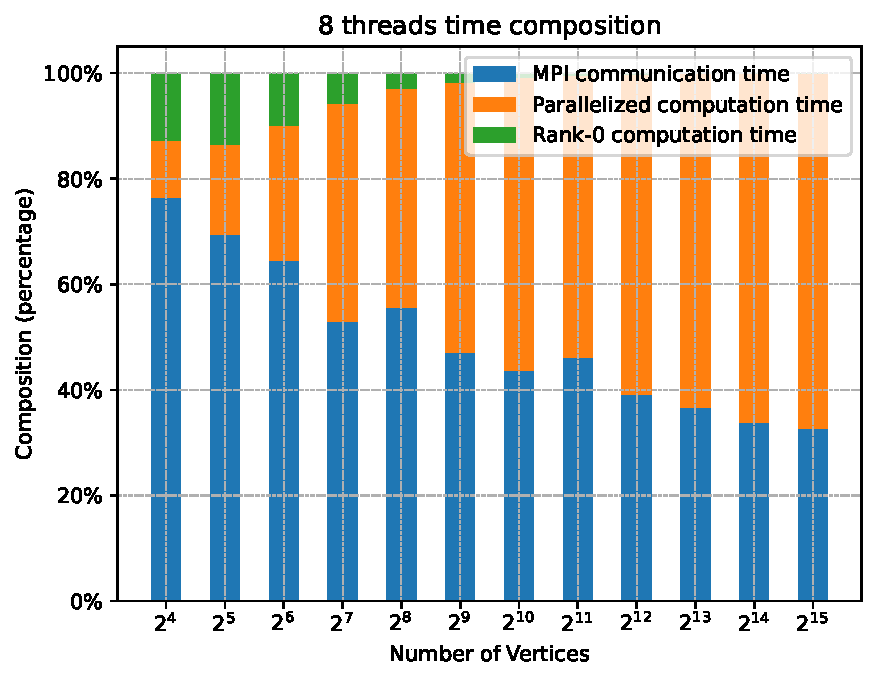
\includegraphics[height=50mm]{./figs/mpi_composition_n1_t8.pdf}
			\caption{8 threads time composition}
			\label{fig:mpi_composition_n1_t8}
	\end{subfigure}
	\begin{subfigure}[b]{0.45\textwidth}
		\centering
		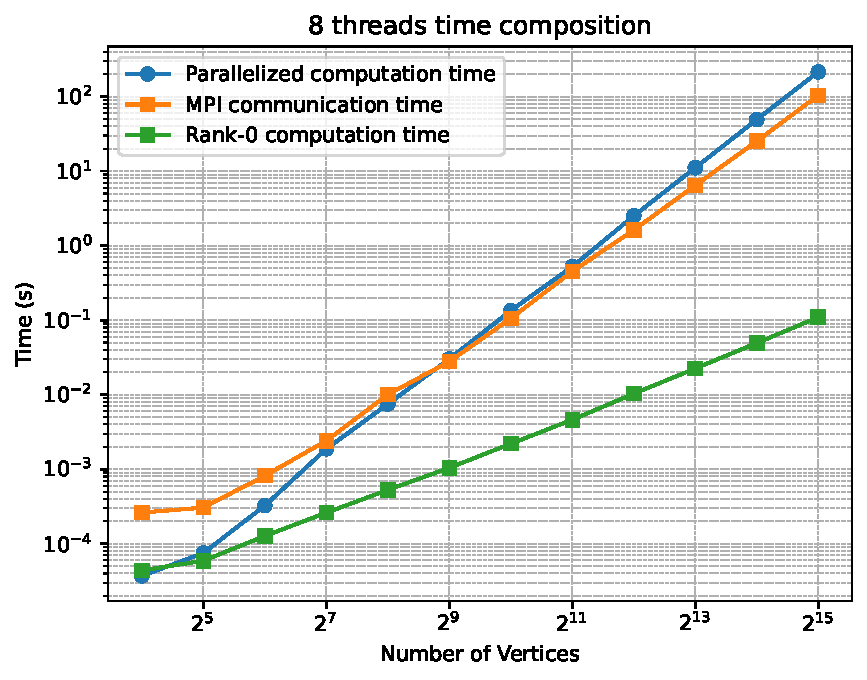
\includegraphics[height=50mm]{./figs/time_n1_t8_composition_time.pdf}
		\caption{8 threads time}
		\label{fig:mpi_n1_t8_time}
	\end{subfigure}
	\vspace{0mm} % Space between rows
	% Bottom row, left (c)
	\begin{subfigure}[b]{0.45\textwidth}
			\centering
			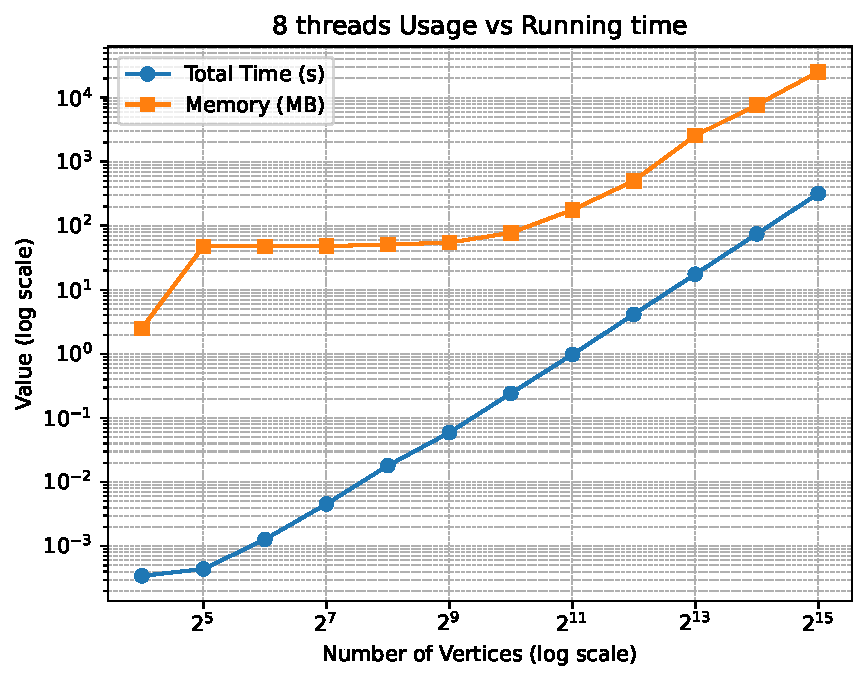
\includegraphics[height=50mm]{./figs/time_mem_n1_t8.pdf}
			\caption{8 threads time and memory usage}
			\label{fig:mpi_composition_n1_t8_time_mem}
	\end{subfigure}
	\hfill
	\begin{subfigure}[b]{0.45\textwidth}
		\centering
		\includegraphics[height=50mm]{./figs/time_mem_n1_t8_table_mem_vs_time.pdf}
		\caption{8 threads time and memory usage table}
		\label{fig:mpi_composition_n1_t8_time_mem_table}
	\end{subfigure}

	\caption{\mstalgo{} with 8 threads}
	\label{fig:mpi_composition_n1_t8_}
\end{figure}

% Composition
% TODO insert round numbers
As the number of vertices on each rank increases, the number of rounds increase as predicted by $O(\log{\log(n)})$. However, the runtime is not benefited much by the slowdown of round growth as shown in \cref{fig:mpi_composition_n1_t8_time_mem} and \cref{fig:mpi_composition_n1_t8_time_mem_table}.

When there are only one or a few vertices on each rank, as the Congested Clique model predicts, the communication time makes up the majority of the total time. And the thread/rank 0 shares the similar fraction of the total time, meaning that there will be at least $10\%$ of time where every other threads remain idle and wait for rank 0 to finish the computation. As we continue to fit larger and larger graphs, the communication time is no longer the majority of. The thread computation starts to take over, and the rank 0 time diminishes \cref{fig:mpi_composition_n1_t8}.

% explain why thread time takes off
The thread time computation time includes everything other than communication and rank 0 computation. Calculating minimum weight edges is a memory bound task. And it is heavily involved in the thread computation time. The memory for the graph grows quadratically with the number of vertices. It means the time spent on preparing the MPI messages also grows accordingly. Further optimization in this algorithm would require more memory efficient data structures.

In the $2^{15}$-vertex example, the expected memory usage is $2^{15} \times 2^{15} \times 4 = 2^{31}$ bytes = $4096$ MB (with double precision). This is much less than the actual memory usage $25251$ MB, meaning the message buffers take the majority of the memory.

% Strong scaling
\begin{figure}[h]
	\begin{subfigure}[b]{0.45\textwidth}
		\centering
		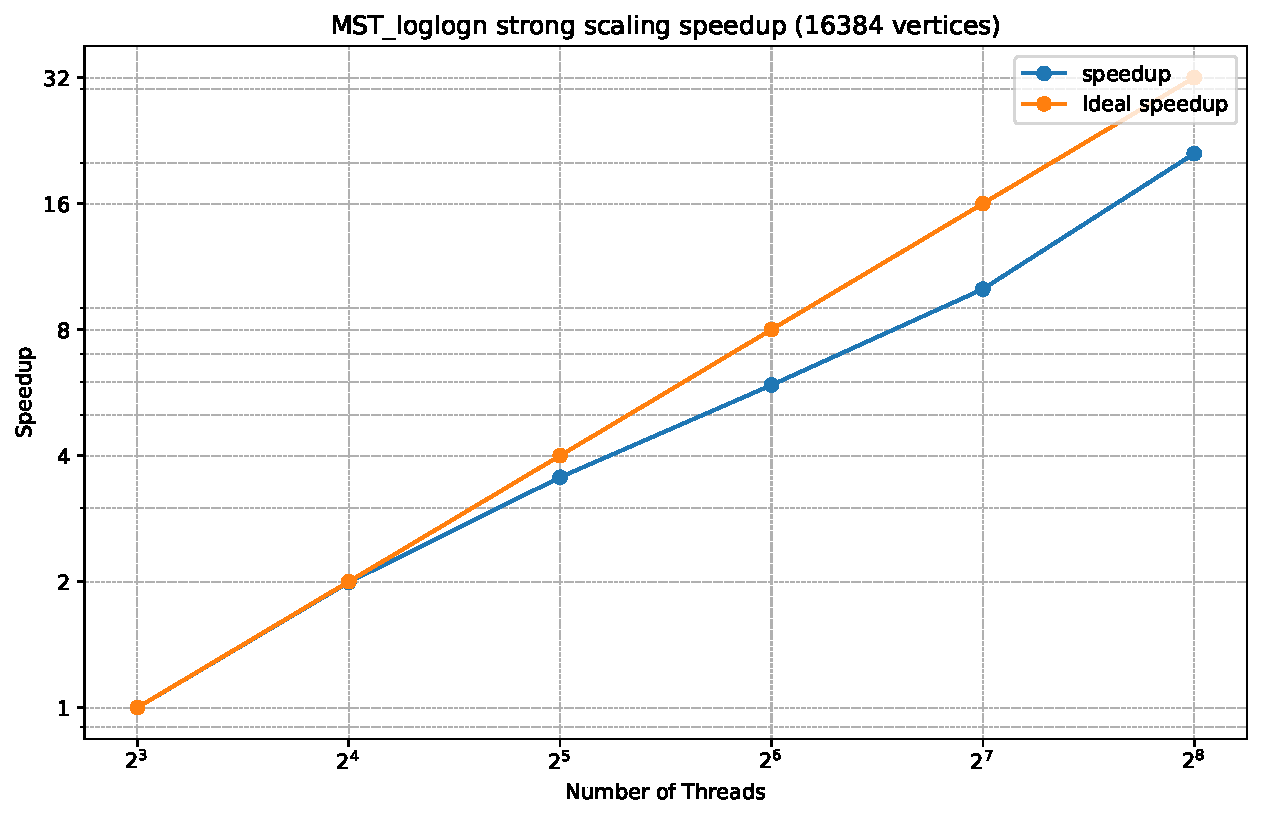
\includegraphics[height=40mm]{./figs/strong_scale_16384_speedup.pdf}
		\caption{16384 vertices strong scaling speedup}
		\label{fig:mpi_composition_strong_scaling_16384_speedup}
	\end{subfigure}
	\begin{subfigure}[b]{0.45\textwidth}
		\centering
		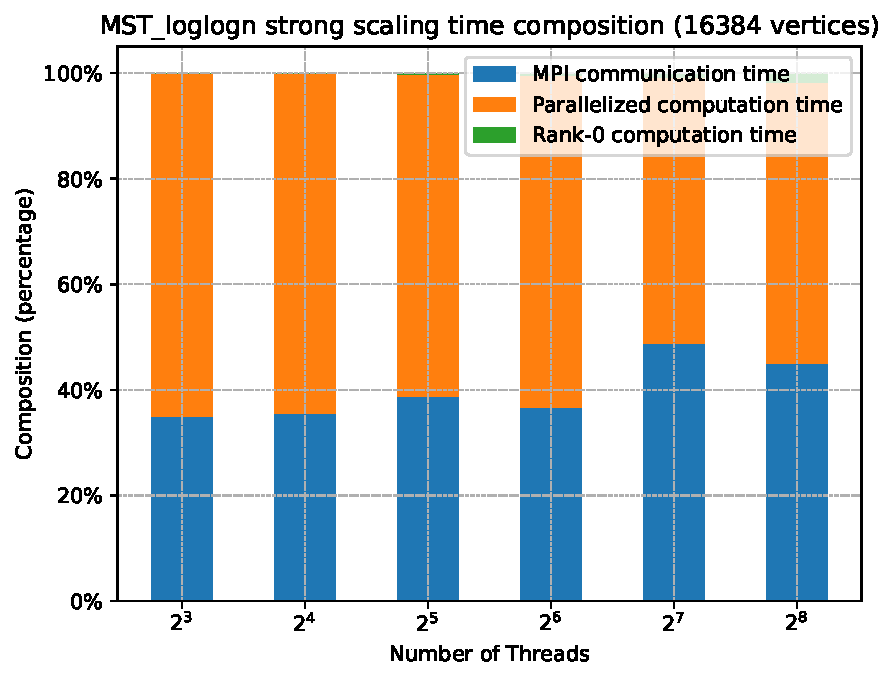
\includegraphics[height=50mm]{./figs/strong_scale_16384_composition.pdf}
		\caption{16384 vertices strong scaling time composition}
		\label{fig:mpi_composition_strong_scaling_16384}
	\end{subfigure}
	\vspace{0mm} % Space between rows
	% Bottom row, left (c)
	\begin{subfigure}[b]{1\textwidth}
		\centering
		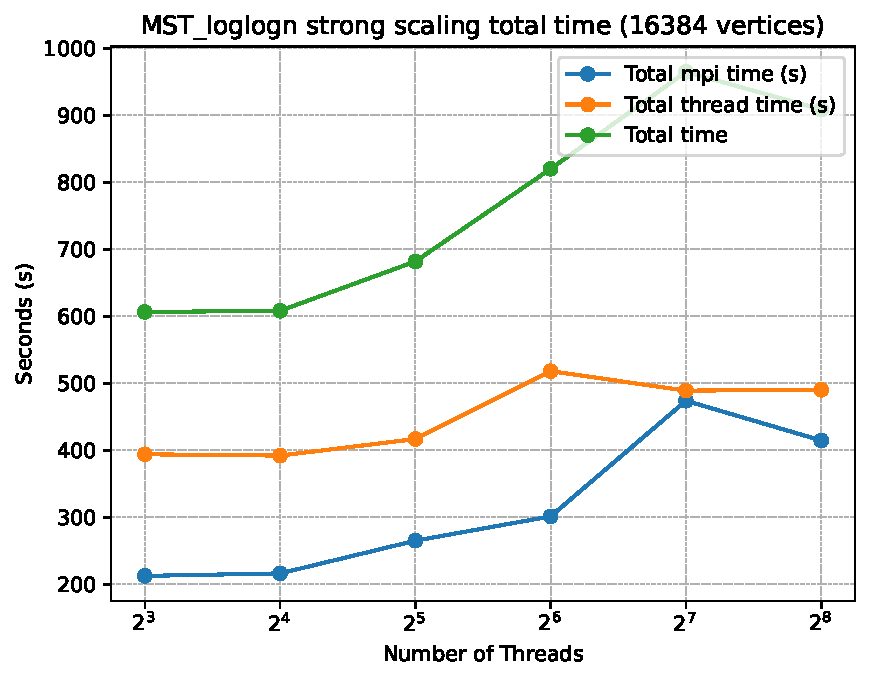
\includegraphics[height=50mm]{./figs/strong_scale_16384_total_time.pdf}
		\caption{16384 vertices strong scaling total time}
		\label{fig:mpi_composition_strong_scaling_16384_total}
	\end{subfigure}
	\label{fig:mpi_composition_strong_scaling_16384_}
\end{figure}

We measure the strong scaling performance of \mstalgo{} on puhti with 16384 vertices and at most 512 CPU threads (as Puhti can provide).

The speedup shown in figure \cref{fig:mpi_composition_strong_scaling_16384_speedup} shows good scalability. It follows the ideal speedup line closely. With 512 threads, it still managed to achieve a speedup over 32 compared to the optimal speed up 64. The thread computation time decreases as the number of threads increases, whereas the communication and rank 0 computation time grow.

\begin{tcolorbox}[colback=white,colframe=black,boxrule=1pt,arc=0pt]
	Key observation: Compute and communication trade-off. Same sized graph, more ranks, less computation time (fraction) per rank (as its averaged out) more communication time (fraction). Vice versa.
\end{tcolorbox}

Figure \cref{fig:mpi_composition_strong_scaling_16384_total} demonstrates that the MPI communication time is the major contributor of the slowdown in speedup. When vertices are partitioned, there will be multiple vertices (nodes in Congested Clique language) on the same thread. Within that group of vertices, no MPI communication is needed. By having more threads and further partitioning the vertices, there are smaller and smaller local groups on threads and that results in more communication need in total, which is why the the scalability of MPI time is poor in the graphs.

On the other hand, the thread computation shows great scalability. The total time remains rather flat in \cref{fig:mpi_composition_strong_scaling_16384_total}

If there were more threads available, there would be a turning point in speedup. However, the number of threads are limited and we can not reach that point. Nonetheless, \mstalgo{} shows good scalability with the number of threads available and great compatibility to vertex partitioning.

\begin{figure}[h]
	\centering
		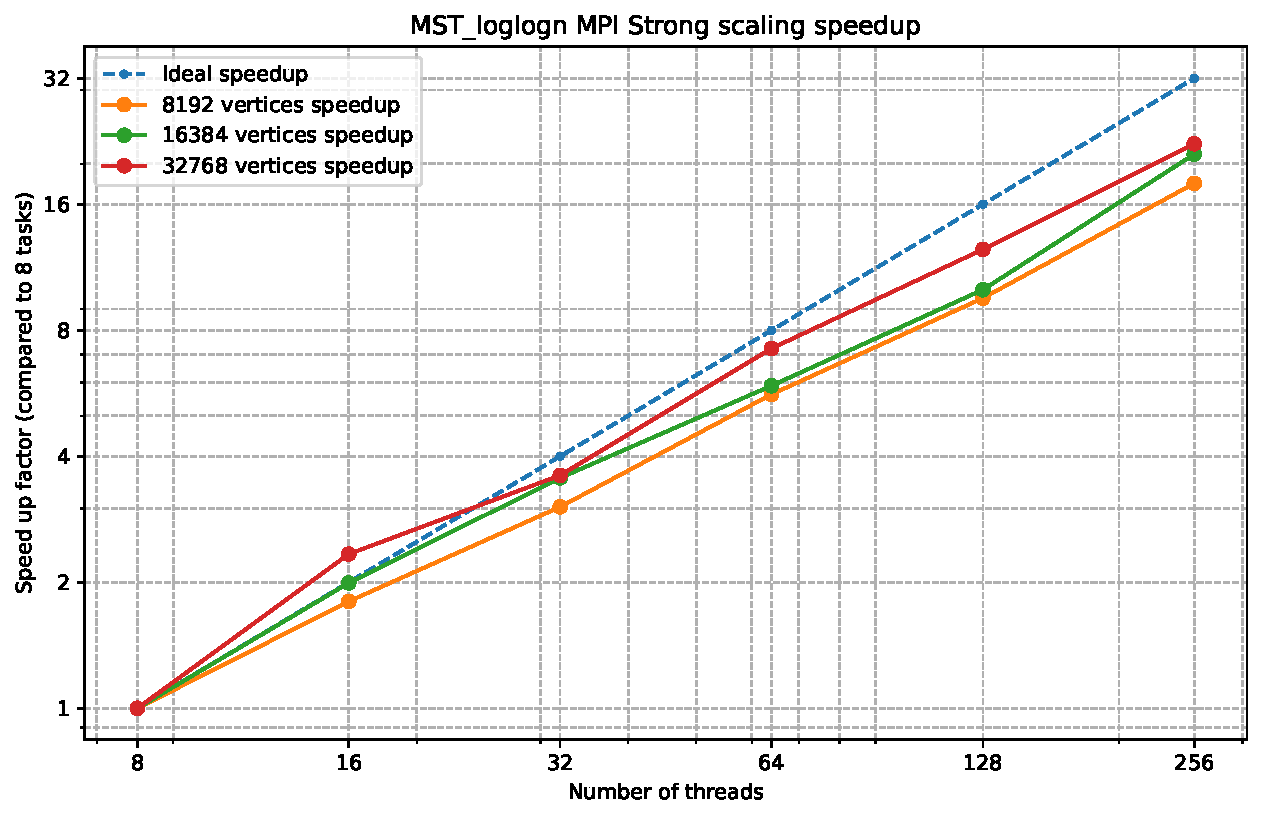
\includegraphics[height=70mm]{./figs/mpi_cpp_strong_scaling.pdf}
	\caption{Strong scaling performance of \mstalgo{}}
	\label{fig:mpi_cpp_strong_scaling}
\end{figure}

Figure \cref{fig:mpi_cpp_strong_scaling} shows the strong scaling performance of \mstalgo{}. There are three different lines in the plot with 8192, 16384, and 32768 vertices. The number of threads increases from 8 to 258 Horizontally. 

All three strong scaling plots are very close to the ideal speedup line. The proportion of execution time spent on the part that can be parallelized is dominant \cite{HPCScaling}. The algorithm scales the best in the strong scaling with 32768 vertices compared to the rest lines, as it is the closest line to the ideal speedup line. The algorithm scales the worst in the strong scaling with 8192 vertices compared to the rest lines, as it is the furthest line to the ideal speedup line. 

From figure \cref{fig:mpi_cpp_strong_scaling}, the larger the graph, the better speedup the algorithm can achieve with the same amount of threads. This result corresponds to the time composition in figure \cref{fig:mpi_composition_n1_t8}. For a fixed amount of threads, more vertices on each thread will lead to more time spent on thread computation and less time on MPI communication and rank 0 computation. 


% % For capacity and the time composition change between thread counts
% \begin{figure}[h]
% 	\centering
% 	% Top row, left (a)
% 	\begin{subfigure}[b]{0.45\textwidth}
% 			\centering
% 			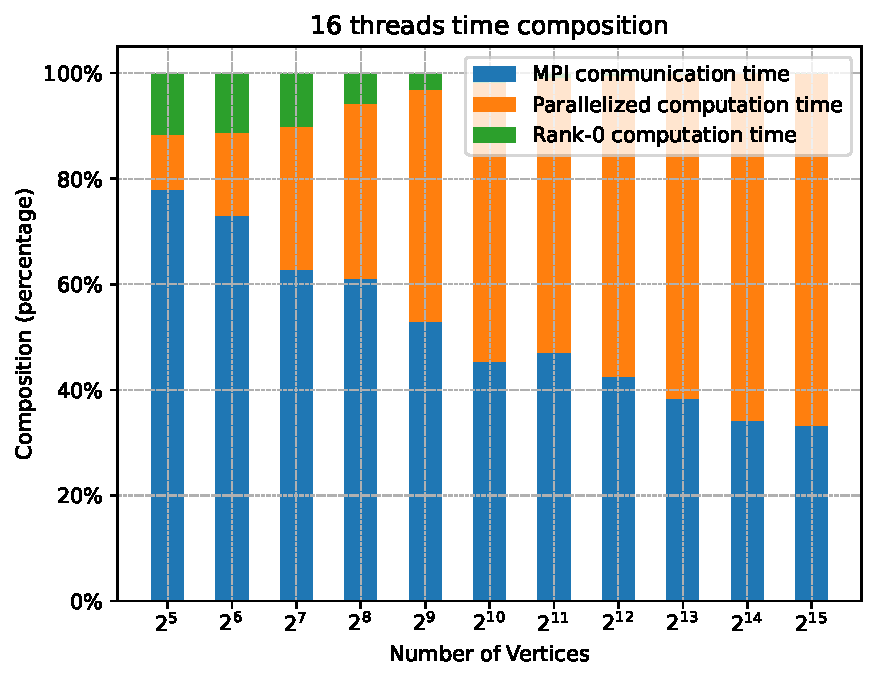
\includegraphics[height=50mm]{./figs/mpi_composition_n1_t16.pdf}
% 			\caption{16 tasks time composition}
% 			\label{fig:mpi_composition_n1_t16}
% 	\end{subfigure}
% 	\hfill
% 	% Top row, right (b)
% 	\begin{subfigure}[b]{0.45\textwidth}
% 			\centering
% 			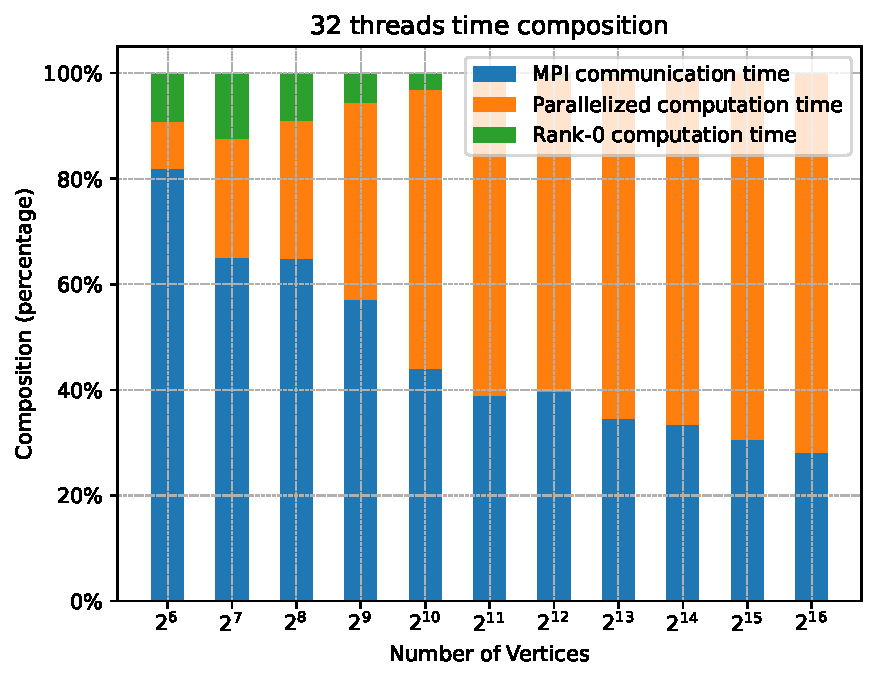
\includegraphics[height=50mm]{./figs/mpi_composition_n2_t16.pdf}
% 			\caption{32 tasks time composition}
% 			\label{fig:mpi_composition_n2_t16}
% 	\end{subfigure}
% 	\vspace{0mm} % Space between rows
% 	% Bottom row, left (c)
% 	\begin{subfigure}[b]{0.45\textwidth}
% 			\centering
% 			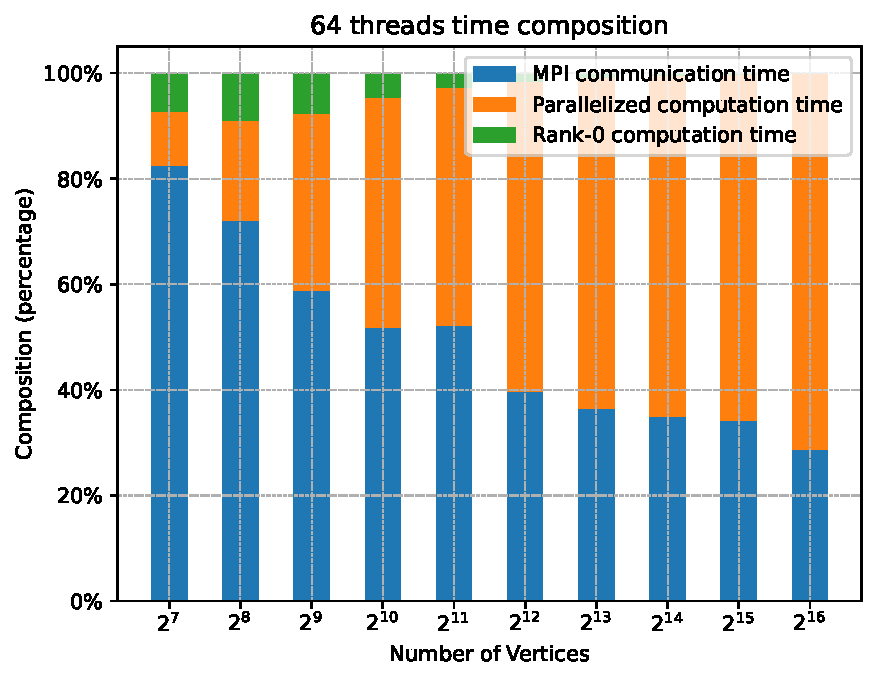
\includegraphics[height=50mm]{./figs/mpi_composition_n4_t16.pdf}
% 			\caption{64 tasks time composition}
% 			\label{fig:mpi_composition_n4_t16}
% 	\end{subfigure}
% 	\hfill
% 	% Bottom row, right (d)
% 	\begin{subfigure}[b]{0.45\textwidth}
% 			\centering
% 			\includegraphics[height=50mm]{./figs/mpi_num_tasks_fraction.pdf}
% 			\caption{MPI task time composition with varying number of tasks}
% 			\label{fig:mpi_num_tasks_fraction}
% 	\end{subfigure}
% 	\caption{\textit{MST} log-log $n$ time composition with more processes}
% 	\label{fig:mpi_composition_grid}
% \end{figure}

% \begin{figure}[h]
% 	\centering
% 		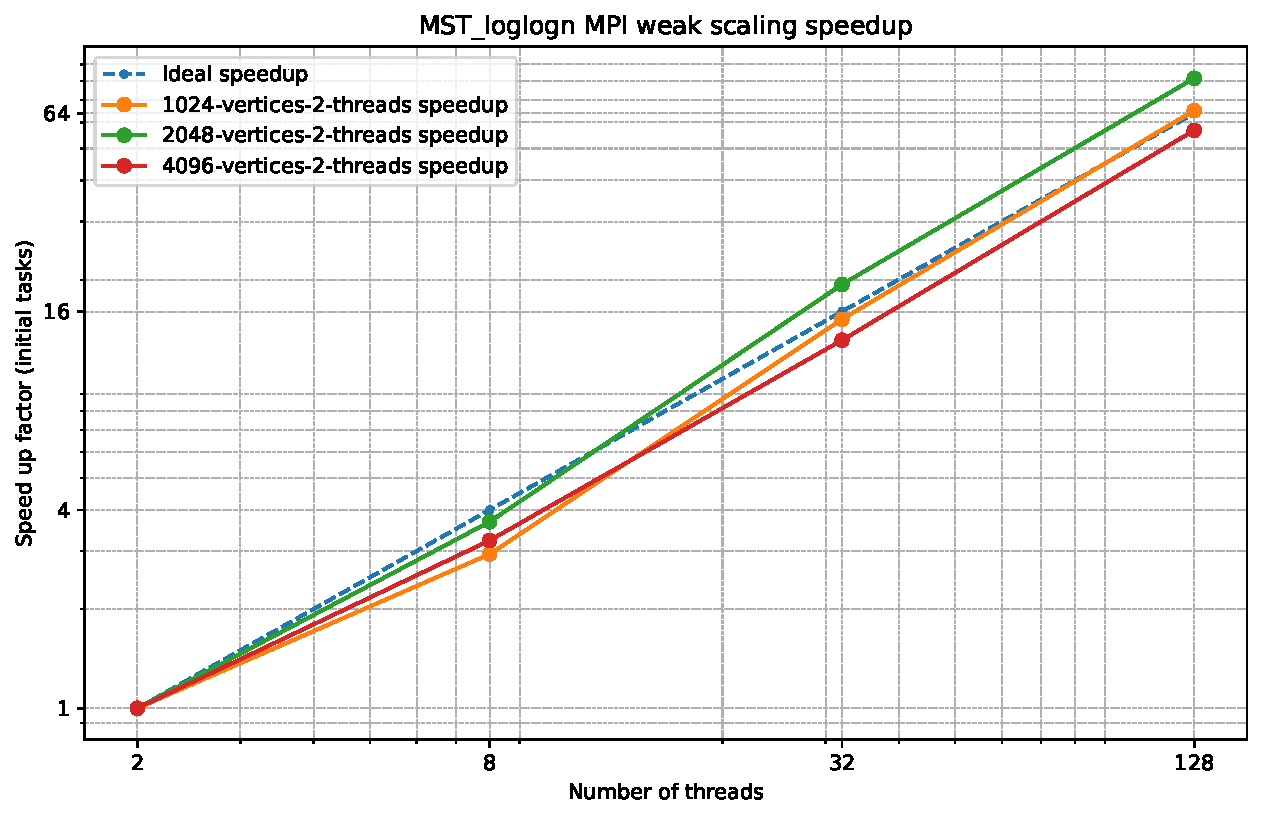
\includegraphics[height=70mm]{./figs/mpi_cpp_weak_scaling.pdf}
% 	\caption{Weak scaling performance of \mstalgo{}}
% 	\label{fig:mpi_cpp_weak_scaling}
% \end{figure}

\subsection{Comparison with prim's algorithm}
\begin{figure}[h]
	\centering
		\includegraphics[height=70mm]{./figs/prim's_vs_A.pdf}
	\caption{Prim's algorithm compared to \mstalgo{} performance}
	\label{fig:prims_vs_A}
\end{figure}
Prim's algorithm is used as the sequential algorithm to compare the performance of \mstalgo{}. It is implemented also in C++ and runs on a single thread on Puhti, with 16G memory.

With 16G memory, prim's algorithm can process 32678-vertex complete graphs (but not 65356), which has $32678 \times 32677 / 2 = 5.33 \times 10 ^ 8$ edges, with 88 seconds. The bottleneck for prim's algorithm to process more edges is to fit the graph to the limited memory of a single node.

Because of the distributed nature of \mstalgo{}, larger graphs can be fit into the memory as the number of threads increases. When working on graphs with the same size, the program needs more memory for MPI's buffer compared to the prim's algorithms.

As shown in \cref{fig:prims_vs_A}, with more than $16$ threads and more, \mstalgo{} is capable of processing 65536-vertex complete graphs (but not 131072). And \mstalgo{} outperforms the prim's algorithm by speed when there are more than $64$ threads.

\begin{figure}[h]
	\centering
		\includegraphics[height=70mm]{./figs/prim's_vs_MST_loglog(n)_single_thread.pdf}
	\caption{Prim's algorithm compared to \mstalgo{} performance with single thread}
	\label{fig:prim's_vs_A_single_thread.pdf}
\end{figure}

When both the prim's algorithm and \mstalgo{} are run on a single thread, the prim's algorithm outperforms \mstalgo{}. The prim's algorithm is more memory efficient and has less computation time. Within the range of the graph size of our work, we see only a minor difference in the time complexity of the two algorithms.
% how well it scales with the number of nodes
% Questioning the time complexity
% bandwidth and optimization
\subsection{Python vs C++}


\begin{figure}[h]
	\centering
		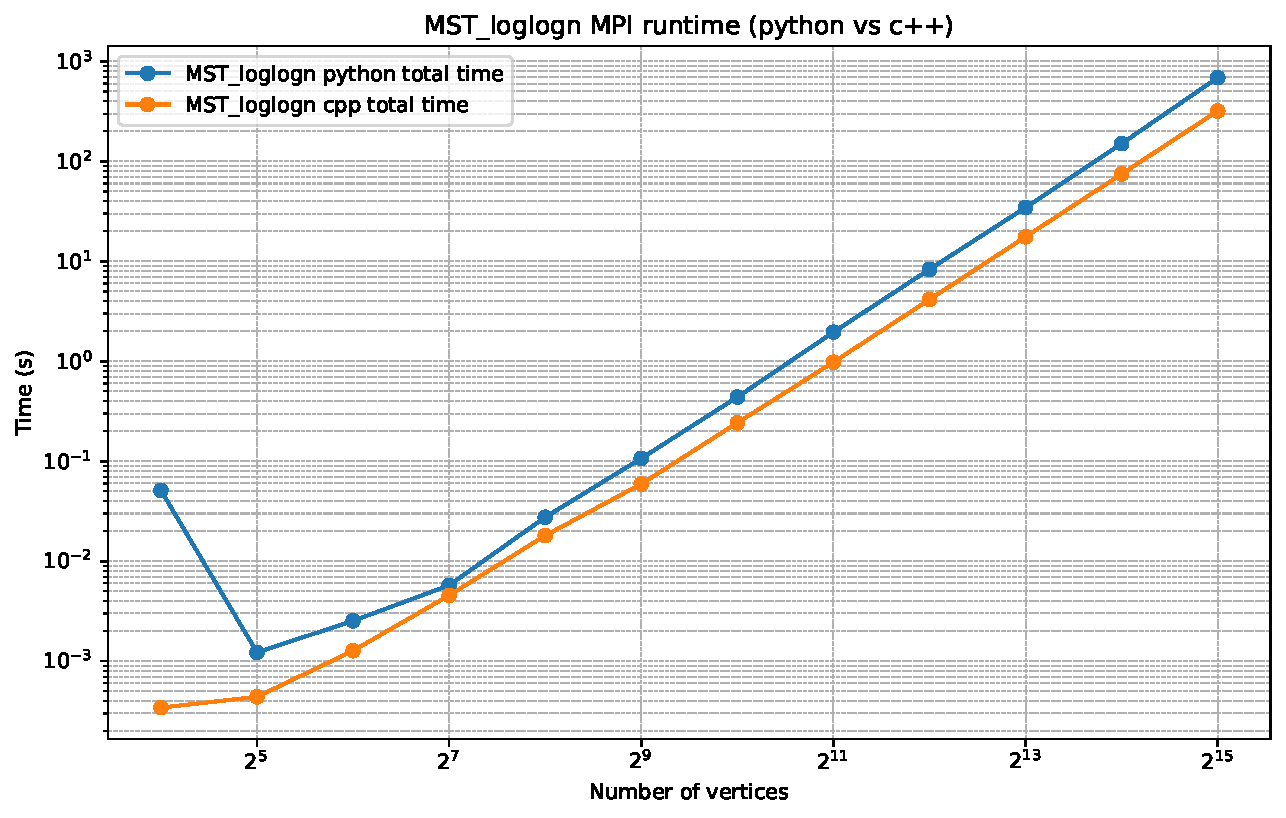
\includegraphics[height=70mm]{./figs/n1_t8_cpp_vs_python_total.pdf}
	\caption{\mstalgo{} Python vs C++ time total time}
	\label{fig:python_cpp_mpi_total.pdf}
\end{figure}

\begin{figure}[h]
	\centering
		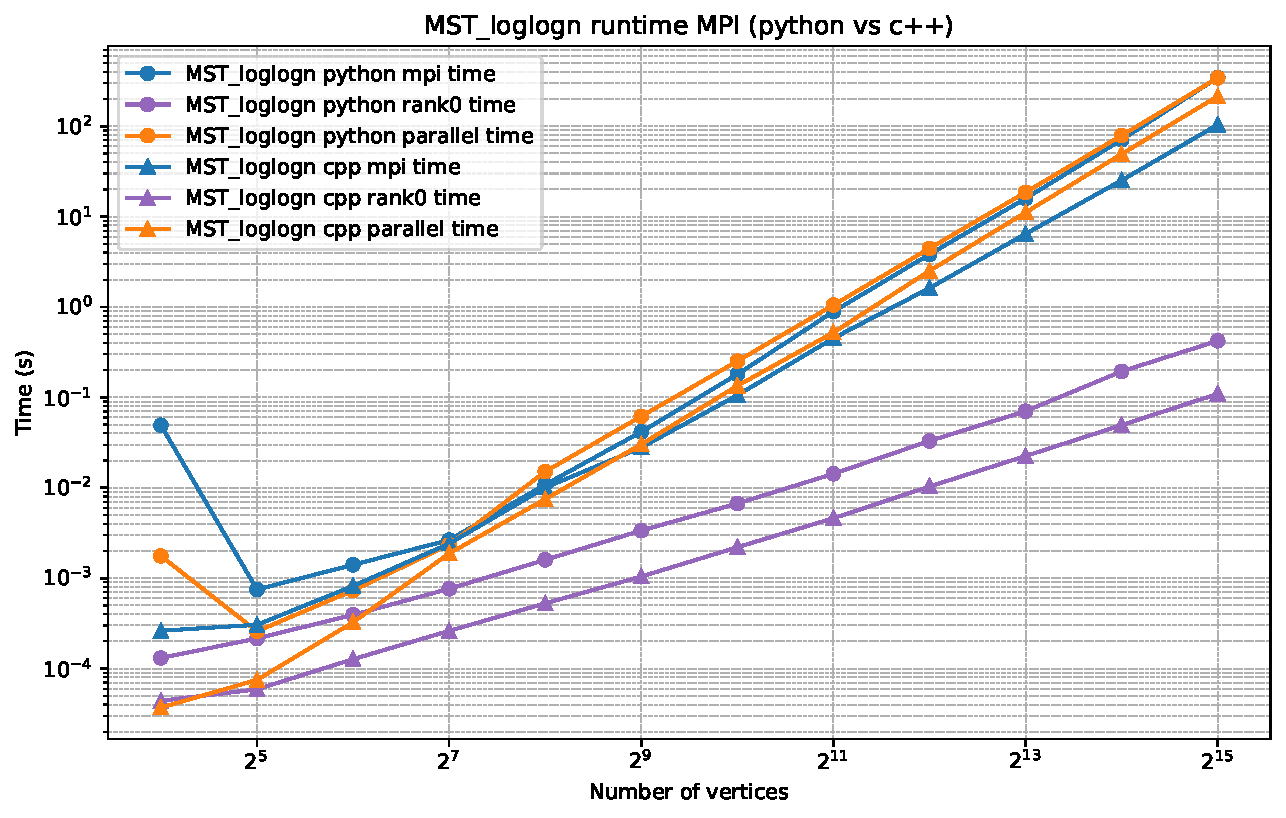
\includegraphics[height=70mm]{./figs/n1_t8_cpp_vs_python_composition.pdf}
	\caption{\mstalgo{} Python vs C++ time composition}
	\label{fig:python_cpp_mpi.pdf}
\end{figure}

The running time difference between the C++ and Python implementation is significant. The slowdown of the Python implementation is majorly contributed by the memory usage of python objects. It takes more time for MPI communication and reading during computation.

When sending messages with $MPI$, the data of an edge is wrapped into an \texttt{Edge} object. The \texttt{Edge} object is composed of a two integers and a double. The two integers indicates the origin and destination of the edge. The double indicates the weight of the edge. In the Python 3.8.0 used in this work, an integer objects takes $28$ bytes, according what \texttt{sys.getsizeof(int())} returns. Python integers are objects of the class \texttt{PyLongObject} \cite{PythonInt}. The class holds auxiliary fields such as \texttt{ob\_refcnt}, \texttt{ob\_size} and \texttt{ob\_digit}, leading to the large size of the integer object. Similar to the integer object, the double object takes $24$ bytes. The large size of the integer and double objects results in the large size of the edge object. The edge object takes $80$ bytes in Python. In contrast, the C++ version of the \texttt{Edge} takes only $16$ bytes. The C++ version of the \texttt{Edge} is a struct composed of two integers and a double. Each integer is \texttt{int32} and the double is \texttt{float64}. There are $128$ bits and thus only $16$ bytes.

The \texttt{Edge} object in python is $5$ times as large as the \texttt{Edge} object in C++. The large size of the \texttt{Edge} object in Python results in the large size of the MPI messages, which yield more time spent on MPI communication as in Figure \cref{fig:python_cpp_mpi.pdf}. More computation time is also expected from Python compared to C++ because of the computation overhead in Python. This is demonstrated in Figure \cref{fig:python_cpp_mpi.pdf}.

Therefore, the total runtime of the Python implementation is significantly larger than the C++ implementation from \cref{fig:python_cpp_mpi_total.pdf}, with the same algorithm and communication framework.
\clearpage

\section{Congested clique with CUDA}
\label{sec:cuda}
% TODO what is a fair comparison with MPI
GPUs are inherently parallel computing devices and more suitable for parallel computing than CPUs. A Nvidia V100 \cite{PuhtiDoc} has 80 streaming multiprocessors. Each is capable of handing 2048 threads at a time, or 64 warps (with 32 threads each warp) \cite{V100Architecture}. A warp is a group of threads that are executed on a Single Instruction Multiple Thread (SIMT) architecture. The threads in a warp execute the same instruction at the same time but on different data \cite{Simtarch}. Multiple warps can be executed at the same time on a streaming multiprocessor grouped into blocks. A streaming multiprocessor can handle one block at a time or multiple blocks concurrently. This architecture allows Nvidia GPUs to issue a large number of threads and execute them in parallel.

Compared to the CPU, the GPU is a device with more lightweight threads and more parallelism. The number of vertices in a Congested clique is comparable to the number of threads that can be issued on a GPU,
which allows the GPU to simulate a node in the Congested Clique model with a thread.

\cref{alg:mst_cuda} describes the pseudo code of the \mstalgo{} implemented with CUDA, "a general purpose parallel computing platform and programming model that leverages the parallel compute engine in NVIDIA GPUs to solve many complex computational problems in a more efficient way than on a CPU" (\cite{CUDA}).
\subsection{Communication}
\begin{algorithm}
	\caption{\textsc{Minimum Spanning Tree} with CUDA}
	\label{alg:mst_cuda}
	\textbf{Require:} Number of vertices $n$, adjacency matrix $\mathbf{A} \in \mathbb{R}^{n \times n}$.\\
	\textbf{On each thread:} Block index $j$, thread index $i$, block dimension $x$, and adjacency sub-matrix $\mathbf{A}[j \times x + i, :] \in \mathbb{R}^{1 \times n}$.
	\begin{algorithmic}[1]
		\State $v \gets j \times x + i$
		\State $T \gets \emptyset$
		\While{there exists $v \notin T$}
			\If{First phase}
				\State \texttt{speed\_up\_kernel()}
			\Else
				\Comment{Step 1}
				\State \texttt{min\_to\_cluster\_kernel()}
				\Comment{Step 2}
				\State \texttt{min\_from\_cluster\_kernel()}
				\Comment{Step 4}
			\EndIf
			\State Perform \textsc{Construct-Frags} and update $T$
			\Comment{Steps 5 and 6}
		\EndWhile
		\State \textbf{Return} the spanning tree $T$

		\State
		\Function{speed\_up\_kernel()}{}
			\State Find the minimum edge $e(v, v')$ connected to $v$
			\State Write the edge to $v_0$
		\EndFunction

		\State
		\Function{min\_to\_cluster\_kernel()}{}
		\State For each fragment $F' \neq F$, compute $e(v, F') \gets \min_{v' \in F'} \{ e(v, v') \}$.
		\State Write all $e(v, F')$ to leaders $l(F')$
		\EndFunction

		\State
		\Function{min\_from\_cluster\_kernel()}{}
		\State For each fragment $F' \neq F$, compute $e(v, F') \gets \min_{v' \in F'} \{ e(v, v') \}$
		\State Perform \textsc{Cheap-Out} and write the edge $e$ $v_0$
		\EndFunction
	\end{algorithmic}
\end{algorithm}

With CUDA, the computation and communication are handled by kernel functions. Kernels functions are functions that are launched to run on the GPU. The threads lives in the context of kernel function. Each  thread simulates one machine in the Congested Clique model, which is a vertex in the clique graph. Each CUDA thread has its own memory space corresponds to the machine memory in the Congested Clique model.

Threads can write and read from the memory space to achieve communication. When thread $A$ sends a message to thread $B$ in the Congested Clique Model, thread $A$ writes the message to the memory space and thread $B$ reads the message from the memory space.

Each kernel function handles only one communication round. This ensures all the communication rounds are synchronized. We don't need barrier with in the kernel. The kernel function exits when all the threads finish their communication and computation. The result of the kernel function resides in the memory space for communication.

The communication is handled in the following way:
\begin{itemize}
	\item[--] step 1: \texttt{min\_to\_cluster\_kernel}
	\item[--] step 2: \texttt{min\_from\_cluster\_kernel} (comm2)
	\item[--] step 3: Buffers are copied to the host
	\item[--] step 4: CPU computation
	\item[--] step 5: The updated cluster info is copied backed in to the Device memory
	\item[--] step 6: Same as above\
\end{itemize}

There are two kernels in algorithm \cref{alg:mst_cuda}, 
namely \texttt{min\_to\_cluster\_kernel} and \texttt{min\_from\_cluster\_kernel}, corresponding to the first and the second steps in \mstalgo{}. Between the two kernel calls, the buffers are not copied back to the host but are kept in the device memory.

When there is only on machine active in step 3, instead of launching a kernel function with a single thread, that part of the computation is done on the CPU. CPU is far more efficient in handling single-threaded computation than the GPU. Thus, we simply write the edge to the memory space of the machine 0 to simulate the gathering process at step 3. Similarly, step 5 and 6 are done by copying the updated cluster information back to the device memory.

\subsection{Memory read and write}
Threads communicate with each other by reading and writing into the vram of V100. When thread $A$ sends a message to thread $B$, thread $A$. For the correctness of the communication, we eliminate the data race scenarios where multiple threads write to the same memory space e.g. when thread $A$ and thread $C$ all send a message to thread $B$.

Two pointers are passed as input arguments into the first kernel \texttt{min\_to\_cluster\_kernel}: \texttt{min\_edges\_bufGPU}, which has all the graph edges with shape $n \times n$ and \texttt{to\_cluster\_bufGPU}, which is the output of the kernel with shape also $n \times n$, where $n$ is the number of vertices in the complete graph. When thread $A$ sends a message to the leader of cluster $F$, it writes the edge to \texttt{to\_cluster\_bufGPU} $[A, leader(F)]$. There are at least $n$ clusters in the graph, so $leader(F)$ never overflows the buffer. One thread send at most one edge to another cluster leader, so each entry in the buffer is a unique space analogous to a link in the Congested Clique model.

With the second kernel \texttt{min\_from\_cluster\_kernel}, two pointers \texttt{to\_cluster\_bufGPU} and \texttt{from\_cluster\_bufGPU} are passed as input arguments. Among them, \texttt{from\_cluster\_bufGPU} is the output of the kernel. It is another $n$ by $n$ buffer. Because at the end of this stage, one cluster will not send more edges than the number of member of the cluster to vertex $0$. There will be at most $n \times n$ edges sent to vertex $0$.

The space of \texttt{from\_cluster\_buf} is arranged in the following way. Each cluster will gets a \texttt{start\_idx} and an \texttt{end\_idx} to indicate the space allocated to the cluster in the array. \texttt{start\_idx} $-$ \texttt{end\_idx} is the number of vertices in the cluster. The \texttt{end\_idx} of cluster $F$ is the same as the \texttt{start\_idx} of cluster $F+1$, making sure the space is not overlapped. This makes up the space for the edges sent to vertex $0$ with the size of maximum $n \times n$.

Finally, rank $0$ or the CPU reads the buffer \texttt{from\_cluster\_buf} and filters out all the edges not \texttt{null} and continues to perform \texttt{Construct-Frags}.

\subsection{Complete and sparse graphs}
% Why sparse graph
The Nvidia V100 GPU has the capability to issue a huge amount of threads but with a limited VRAM of $16G$ / $32G$. The total memory can be used is much lower than the previous MPI simulation of $8G$ / $16G$ per thread. Compared to the MPI implementation, V100 can only store much less edges in the memory, even it has the capability to launch a large quantity of threads for vertices. A V100 can issue $2048$ threads on each streaming multiprocessor, which is $80 \times 2048 = 163840$ threads in total. We walk around this limitation by introducing sparse graphs. Sparse graphs saturate the GPU's thread capability better by having less edges on each vertex. In this way, the computation is better balanced among the threads.

In the Congested Clique, the network graph is the equivalent as the graph to be solved, which is a complete graph / network. Each vertex / thread, has a list of weight of adjacent edges in memory. In the sparse graph setting, each vertex has a varying number of adjacent edges. The edges of the graph are represented as a adjacent list when generated. The network remains fully connected in the sparse graph setting, meaning any thread and send message to any other threads.

\mstalgo{} works on the sparse graph as well.
% adjacency list/matrix
In memory, a complete graph is represented by an adjacency matrix, where each column represents the adjacent edges of a vertex. Whereas the sparse graph is represented by an adjacency list due to the varying rank of each vertex. Each vertex has a list of adjacent edges.

% Why the algo works on sparse graph
\begin{tcolorbox}[colback=white,colframe=black,boxrule=1pt,arc=0pt]
	\mstalgo{} is designed to work on a complete graph but it does work for connected spares graphs as well.

	\textbf{Proof}: A sparse graph $G$ is analogous to a complete graph $G'$ with weight of edges which are disconnected in the sparse graph set to infinity. \mstalgo{} is capable of finding the MST in $G'$. The edges with infinite weight will not be picked in step 4 for $G'$, meaning they can be removed from the candidate list of step 4. Same for the previous steps. As the network remains fully connected, the infinite weight edges will not affect the communication. Thus, the edges with infinite weight can be ignored in the computation to form a sparse graph.
\end{tcolorbox}

To generate a connected sparse graph, the following steps are taken.
\begin{itemize}
	\item[--] Generate a Prüfer sequence with all the vertices. A Prüfer sequence is an unique sequence of vertices that encodes a tree \cite{Prufer1918}. The tree serves as the skeleton of the sparse graph making sure the graph is connected.
	\item[--] Convert the Prüfer sequence into a tree.
	\item[--] Add edges to the tree randomly until the expected rank is met.
\end{itemize}

\subsection{Best practices}
Similar practices used in the MPI implementation are used on the CUDA implementation to ensure a relatively fair comparison.
% list
\begin{itemize}
	\item[--] The constructed MST is maintained as a union-find data structure.
	\item[--] Same edge objects and weight datatype are used in the CUDA implementation as in the MPI implementation.
	\item[--] The simplification on the first phase is applied.
\end{itemize}

\subsection{Profiling}
To accurately measure the performance of the CUDA implementation, we need to profile the program. The profiling is done with nvprof, a command-line profiler provided by Nvidia. The profiling result shows the time spent on the memory copying and the kernel functions. The time spent on each kernel function is the time spent on the communication and local computation in each round.

\clearpage

\section{Performance with CUDA}
\label{sec:cuda_performance}
\subsection{Conclusion overview}

\begin{itemize}
	\item CUDA implementation of \mstalgo{} demonstrates significant speedup compared to single-threaded Prim's algorithm, leveraging the GPU's parallelism.
	\item The communication between threads is efficiently handled using memory read and write operations, analogous to message passing in the Congested Clique model.
	\item The time spent on kernel execution scales well with the number of vertices, but memory operations and CPU computation become bottlenecks as graph size increases.
	\item Sparse graphs show potential for better workload balancing on GPUs, but the overhead of adjacency list operations can negate performance gains.
	\item Smaller block sizes improve workload distribution among Streaming Multiprocessors (SMs), reducing kernel execution time.
	\item CUDA implementation is limited by GPU memory capacity, making it challenging to handle large complete graphs without sparsity.
\end{itemize}

% 1. How is the read and write analogous to the communication. How much time it takes? Is it the majority of the time? How does divergence affect the performance (Check the assembly maybe)?

% 2. How much time does rank 0 time take compared to the gpu time? Will it become the bottleneck at some point?

% 3. Does sparse graph promote better workload balancing?

% 4. Is it fair to compare with MPI? Can we fit equal large graphs into the memory? MPI vs single V100 why?

% 5. Compared with a single threads Prim's, can we beat it? (Compare the theoretical peak flops and the actual flops, are we utilizing the hardware well?)

% 6. How well does the algorithm scale with the number of threads? (Can we scale further with MPI?) (Optional)

% 1024 / 2048 per block what's the diff.
% What to compare (CPU single thread? why not)
\subsection{Performance}
% TODO 1, 2, 4, 6
\begin{tcolorbox}[colback=white,colframe=black,boxrule=1pt,arc=0pt]
As shown in the figure, DtH refers to the initial data transfer from the host to the device. This operation scales proportionally with the graph size, as the entire graph data must be copied to the GPU memory. Conversely, HtD represents the final data transfer from the device back to the host, which scales at a slower rate due to the reduced amount of data being transferred.

Within the kernels, each thread simulates a machine in the congested clique model. At the beginning of each round, threads are responsible for receiving messages, which corresponds to reading from the buffer. Subsequently, threads process the received data and send their own messages, which involves writing to a new buffer.

The workload on the \texttt{to\_cluster\_kernel} is notably larger than that on the \texttt{from\_cluster\_kernel}. This is because, at the start of the algorithm, there are significantly more edges to process, resulting in a higher computational demand for the \texttt{to\_cluster\_kernel}.
\end{tcolorbox}

\begin{figure}[h]
	\begin{subfigure}[b]{0.45\textwidth}
		\centering
		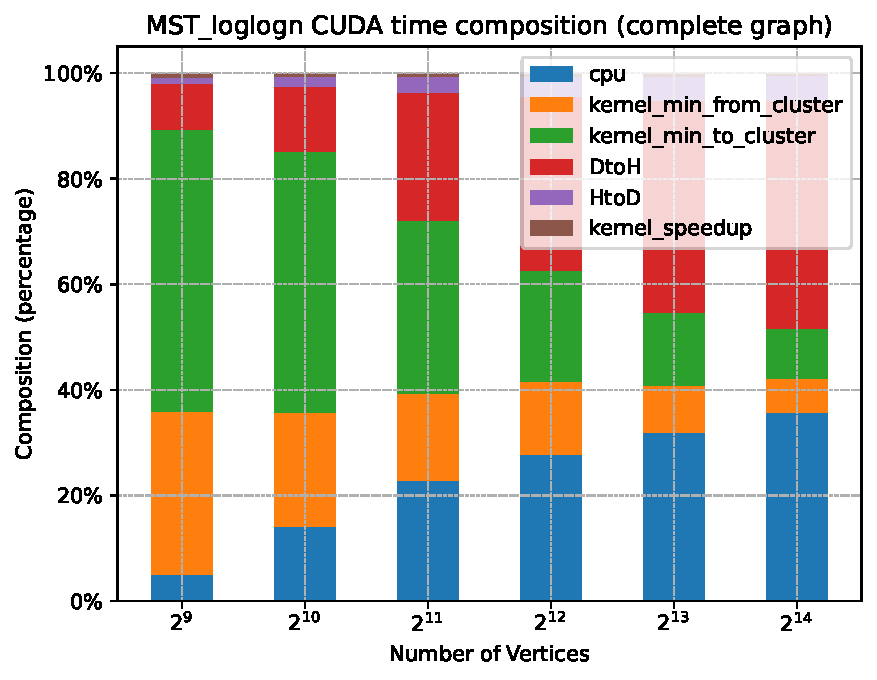
\includegraphics[height=50mm]{./figs/cuda_composition_complete.pdf}
		\caption{\mstalgo{} CUDA time composition with complete graph}
		\label{fig:cuda_composition_complete.pdf}
	\end{subfigure}
	\begin{subfigure}[b]{0.45\textwidth}
		\centering
		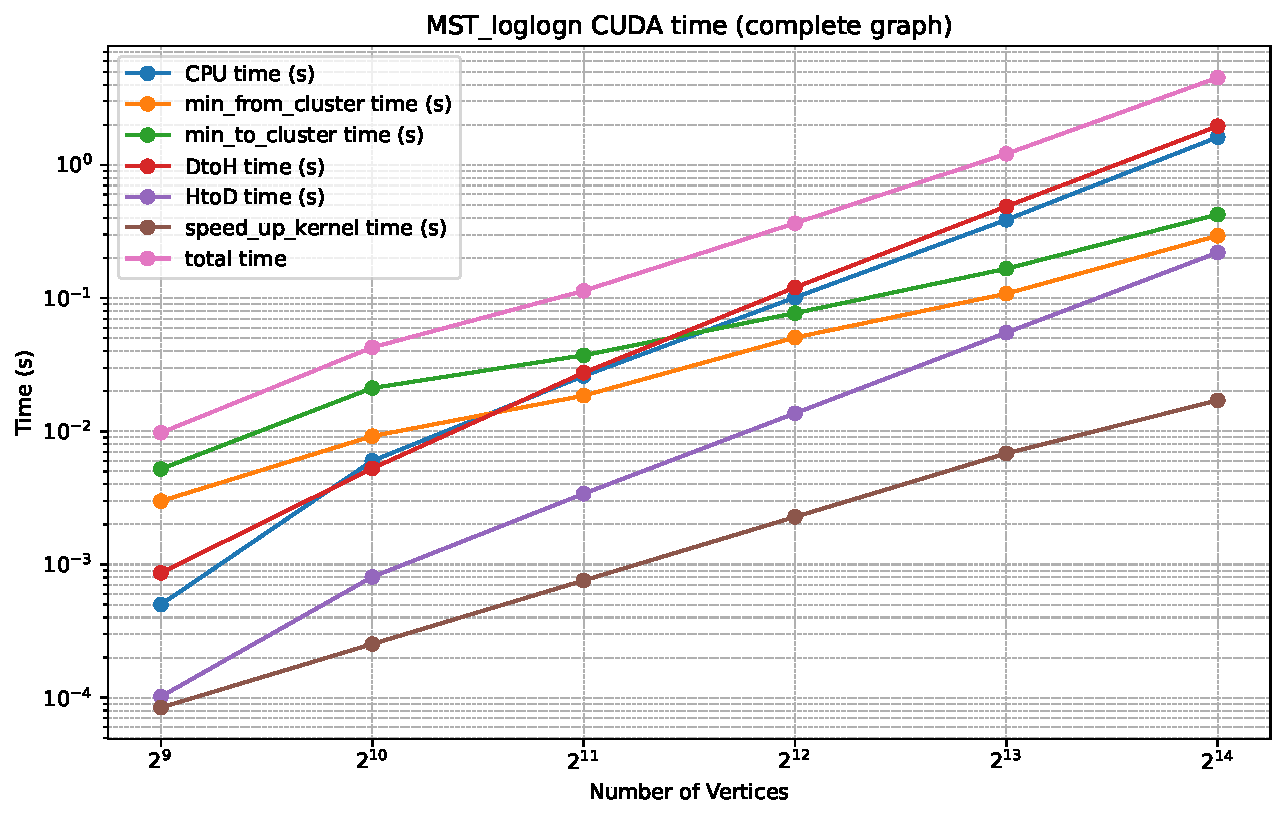
\includegraphics[height=50mm]{./figs/cuda_composition_complete_time.pdf}
		\caption{\mstalgo{} CUDA time with complete graph}
		\label{fig:cuda_composition_complete_time.pdf}
	\end{subfigure}
	\caption{\mstalgo{} CUDA time composition with complete graph. Each block has 1024 threads, each thread simulates a vertex.}
	\label{fig:cuda_composition_complete}
\end{figure}

We run the CUDA implementation \cref{alg:mst_cuda} on Puhti with a Nvidia V100 GPU. There are massive amount of thread resources on one V100. The workload of complete graphs are not able to saturate the thread resources before the vram is full. \cref{fig:cuda_composition_complete} shows the time composition and total time of the CUDA implementation with complete graphs. The number of vertices scales from $2^{9}$ to $2^{14}$. Considering the communication buffers used in the program, $2^{14}$ is the largest graph that can be fit into the vram of a V100. The number of threads in each block is $1024$.

Because the maximum amount of threads can be issued is around $2^{26}$ on V100, Every vertices can be mapped to a thread during the scaling. Compared to the $|E|$ of the graph, which scales quadratically with the number of vertices, the workload among the threads scale linearly within the kernel. However, having the workload scales linearly in the kernels doesn't mean it scales linearly throughout.

\cref{fig:cuda_composition_complete_time.pdf} shows the time of each kernel, memory operation, CPU and total time of the program as the number of vertices increases. The time of \texttt{min\_to\_cluster\_kernel} and \texttt{min\_from\_cluster\_kernel} increases noticeably slower compared to other time categories. On contrast, the time of memory operations and CPU computation increases noticeably faster. The workload for them can not be distributed to more work units like with the kernels. Thus they scale corresponds to $|E|$.

% Composition change
From \cref{fig:cuda_composition_complete.pdf}, we see the composition changes during the scaling. As explained earlier, The CPU time and memory copying time remain insignificant when the number of vertices is small, but as the number of vertices increases, these times become more prominent. Eventually, the kernels time is insignificant, and the nonparallelizable part of the program contributes over $80\%$ of the total time, when graph size reaches $2^{14}$ vertices.


\begin{figure}[h]
	\centering
		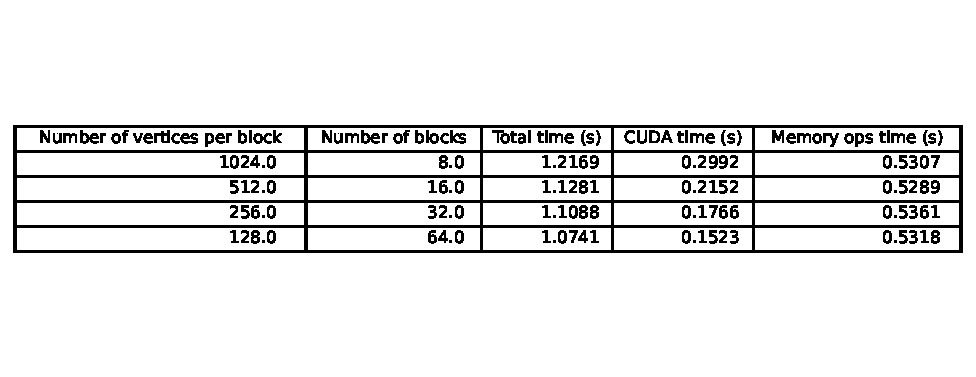
\includegraphics[height=45mm]{./figs/cuda_complete_varying_block_size_8192.pdf}
	\caption{\mstalgo{} CUDA time with complete graph with varying block size}
	\label{fig:cuda_complete_varying_block_size_8192.pdf}
\end{figure}

However, the CUDA time can be further reduced by having smaller block sizes, when the SMs are not well saturated. \cref{fig:cuda_complete_varying_block_size_8192.pdf} shows the time of the CUDA implementation with complete graphs with $8192$ vertices and varying block sizes. The number of vertices is fixed to $8192$. The time of the program decreases as the block size decreases. The time of the program is the lowest when the block size is $256$. The time of the program increases when the block size is further decreased.

Going from block size $1024$ to $128$, the CUDA time is reduced almost by half. More blocks are launched with smaller block size, which means more SMs are utilized. The reduction in time is from the less warps on each Streaming Process (SP), going from $32$ to $4$ warps with $32$ threads in each warp. When there are SMs idling, this is a good way balancing the workload among the SMs.

% small conclusion??

\subsection{Complete vs sparse graph}

\begin{figure}[h]
	\begin{subfigure}[b]{0.45\textwidth}
		\centering
		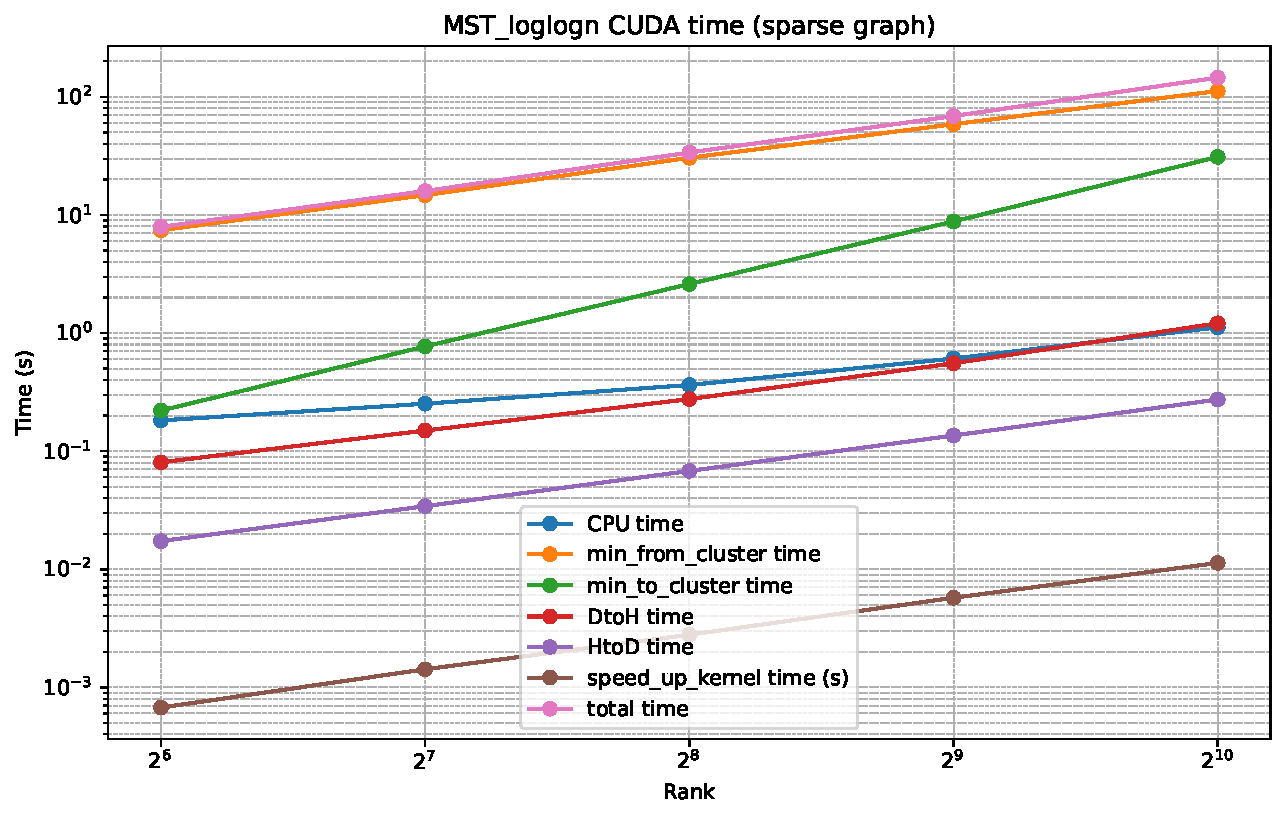
\includegraphics[height=40mm]{./figs/cuda_composition_sparse_time.pdf}
		\caption{\mstalgo{} CUDA time composition with sparse graph}
		\label{fig:cuda_composition_sparse_time.pdf}
	\end{subfigure}
	\begin{subfigure}[b]{0.45\textwidth}
		\centering
		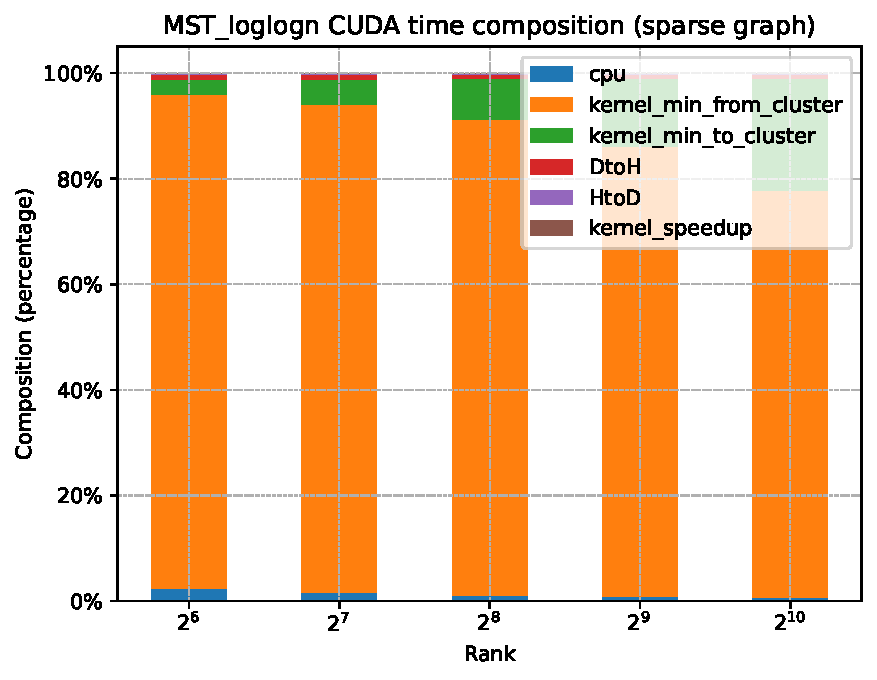
\includegraphics[height=45mm]{./figs/cuda_composition_sparse_persistent.pdf}
		\caption{\mstalgo{} CUDA time with complete graph}
		\label{fig:cuda_composition_sparse_persistent.pdf}
	\end{subfigure}
	\caption{\mstalgo{} CUDA time composition with sparse graph. There is a block on each SM and each block has 1024 threads/vertices.}
	\label{fig:cuda_composition_sparse}
\end{figure}

We modified \cref{alg:mst_cuda} to work with sparse graphs. The algorithm itself works out of the box with sparse graph. But the buffer allocation and accessing need to be modified to comply with the sparsity. Each SM possess $1024$ vertices with $1024$ threads, resulting in $80 \times 1024 = 81920$ vertices in total in the sparse graph. \cref{fig:cuda_composition_sparse_time.pdf} shows the time of the CUDA implementation with sparse graphs. The x-axis is the average rank of the sparse graph, which goes from $64$ to $1024$.

However, the time of the CUDA implementation with sparse graphs is even larger than the time of memory operations and CPU computation. Whereas in the complete graphs, the time of the CUDA implementation is smaller than the time of memory operations and CPU computation. This is the exact opposite of the expectation. Most of the slow down is caused by the data structure overhead from the sparse graph. Because of the sparsity of the adjacent list. When you access the adjacent list, you have to loop through all the edges to find the edge to vertex $v$. This is a $O(n)$ operation. The time of the kernel is $O(n^2)$ in the worst case.  And there are more clusters at the beginning which means more workload in the kernel. Thus in \cref{fig:cuda_composition_sparse}, the kernels are taking the most time, and \cref{fig:cuda_composition_sparse} the sparse graph is slower than the complete graph with the same amount of edges.

\begin{figure}[h]
	\centering
		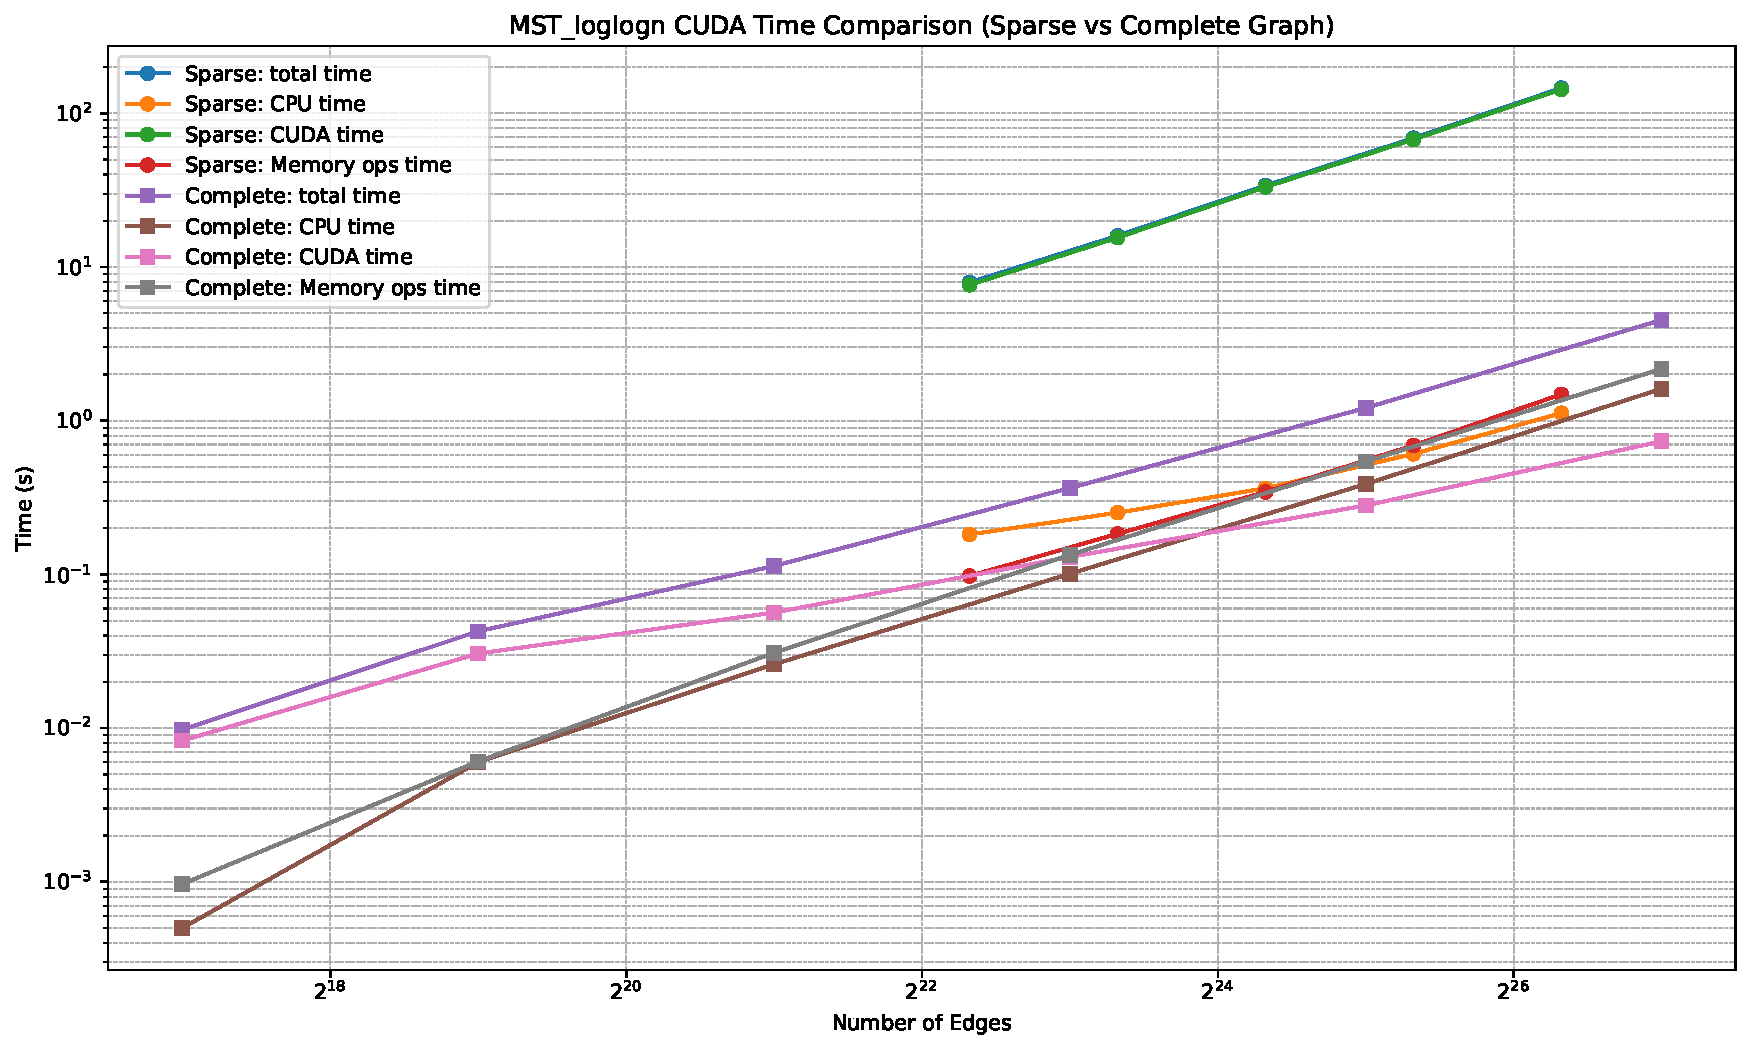
\includegraphics[height=70mm]{./figs/cuda_composition_comparison.pdf}
	\caption{\mstalgo{} CUDA time comparison with complete and sparse graph}
	\label{fig:cuda_composition_comparison.pdf}
\end{figure}

In the kernel \texttt{min\_from\_cluster\_kernel}, there a nested loop

% More clusters (inner loop. more time in from edges the kernels)
% We don't know where is the edge to v for example in the buffer. We have to loop through all the edges to find the edge to v. 
% Number of clusters: 4093
% Number of clusters: 162
% Number of clusters: 1

% Number of clusters: 20512
% Number of clusters: 725
% Number of clusters: 1

% N^2 loop in the to cluster so faster growth.
%  it didn't take more rounds in the end. 2 rounds

\subsection{Comparison with Prim's on single threaded CPU}
\begin{figure}[h]
	\centering
		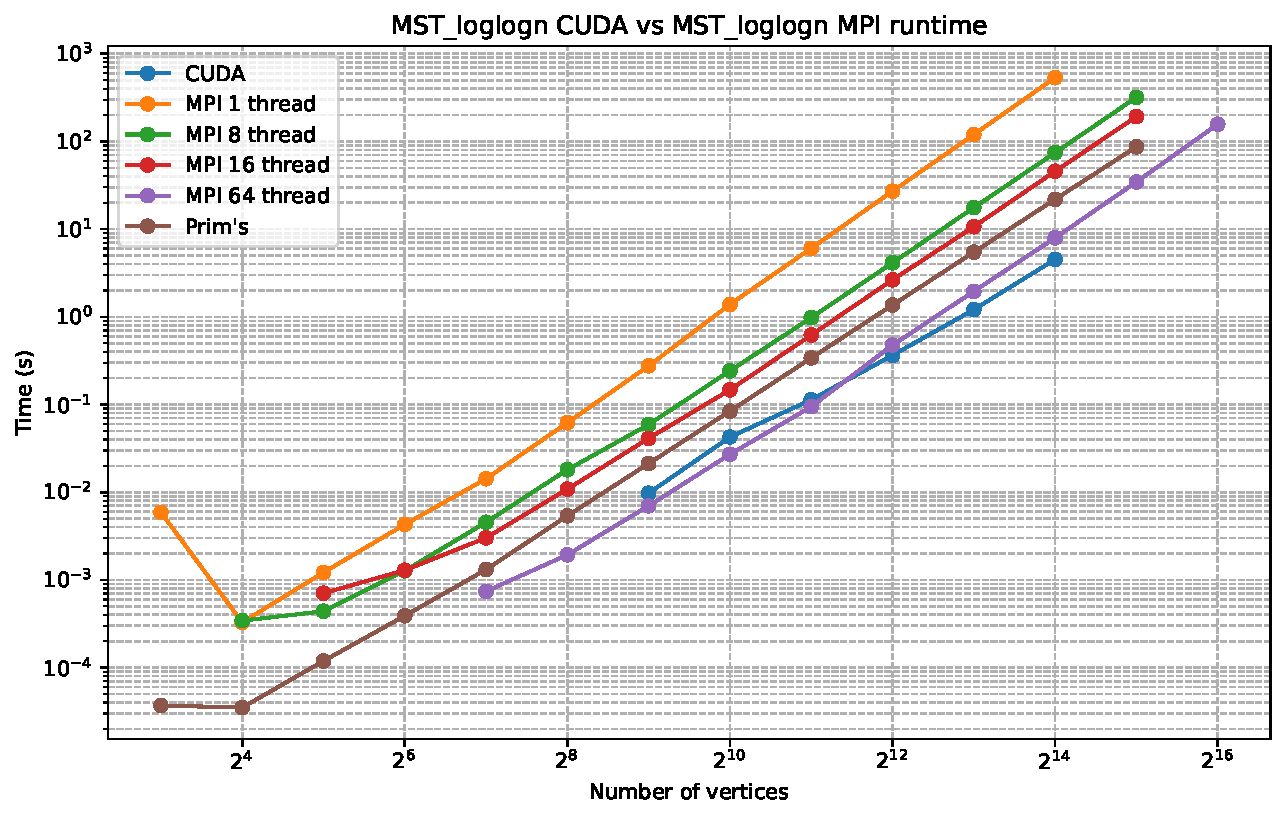
\includegraphics[height=70mm]{./figs/CUDA_vs_MPI.pdf}
	\caption{\mstalgo{} CUDA time comparison with MPI and Prim's algorithm}
	\label{fig:CUDA_vs_MPI.pdf}
\end{figure}

Compared with the vanilla Prim's algorithm, the CUDA implementation is significantly faster, with a slower grow in time as the graph size grows, according to \cref{fig:CUDA_vs_MPI.pdf}. While the single-threaded MPI implementation is the slowest, it beats the prim's algorithm when the number of threads is larger than $64$. With $64$ threads, the performance is comparable to the CUDA implementation but with steeper slope.
\clearpage
\section{Conclusion}
\label{sec:conclusion}
When simulating the Congested Clique model with MPI on CPU threads, limited thread resources necessitate vertex partitioning. With few vertices per rank, communication time dominates, but as graph size increases, computation time becomes the bottleneck. Comparing \mstalgo with Prim's algorithm, \mstalgo requires more compute and memory but outperforms Prim's in wall clock time with more work nodes and handles larger graphs. The bottleneck for larger graphs is MPI message memory. The number of rounds is $O(\log{\log{n}})$, as predicted. Python is significantly slower than C++ due to larger memory usage for MPI messages and slower computation, making it more memory-bound.

The high parallelism of the GPU makes it good at parallelize the vertex workload very well. The assignment of the vertex to the thread is very natural. However, when comes to clique graphs, how to fit graphs into vram is a challenge. The high parallelism can be underutilized if the graph is too large to fit into the vram. Sparser graphs show better affinity to the memory-compute trade-off of the GPU.

However, Congested Clique algorithms are often not optimized to run on GPUs. The computation paradigm shows characteristics of CPU computation. Branching in the algorithms brings divergence among the threads on the same SIMT unit, potentially causing the performance to degenerate. Moreover, it is not intuitive to implement the communication between threads. Is it often required that one thread is globally accessible by another even if they are not in the same block. With this constraint, is it not intuitive how to utilize the shared memory of the block. We have to read and write to the vram, which is designed to be slower than the shared memory. We are also missing some matrix operations that are common in the GPU programming, such as MFMA, MMA operations, and their underlying hardware support such as tensor cores.

TODO insert more CUDA conclusion here.

\clearpage
\section{Future work}
\label{sec:future}
How different datatypes affect the performance. We tried double precision, but how about single precision? Hardware typically have different support on different datatypes. E.g. on GPU, single / half precision has better support than double precision.

Can we optimize the algorithm to comply with the GPU architecture better? E.g. how to utilize the shared memory better? How to reduce the divergence among the threads? How to utilize the tensor cores?

\clearpage
%% Bibliography/ list of references
%%
\thesisbibliography

\begin{thebibliography}{99}

	\bibitem{MSTLogLogn} 
	Zvi Lotker, Boaz Patt-Shamir, Elan Pavlov, and David Peleg, "MST Construction in $O(\log{\log{n}})$ Communication Rounds," 
	\textit{SIAM Journal on Computing}, vol. 35, no. 1, pp. 120–131, 2005. 
	\url{https://doi.org/10.1137/S0097539704441848}
	
	\bibitem{powerCongestClique} 
	M. Ghaffari, F. Kuhn, and C. Lenzen, "On the power of the congested clique model," 
	\textit{Proceedings of the 2013 ACM Symposium on Principles of Distributed Computing (PODC '13)}, pp. 367–376, 2013. 
	\url{https://www.researchgate.net/publication/266659337_On_the_power_of_the_congested_clique_model}
	
	\bibitem{Puhti} 
	"Puhti supercomputer," CSC - IT Center for Science. 
	\url{https://research.csc.fi/-/puhti}
	
	\bibitem{PuhtiService} 
	"Puhti Service Description," CSC - IT Center for Science, Jun. 2021. 
	\url{https://research.csc.fi/documents/48467/640068/Puhti-servicedescription-0621.pdf/e6fd32ae-92ea-2d42-0b6c-9f73c1a4c418?t=1628595451763}
	
	\bibitem{PuhtiDoc} 
	"Puhti Computing Systems," CSC - IT Center for Science. 
	\url{https://docs.csc.fi/computing/systems-puhti/}
	
	\bibitem{Slurm} 
	"Slurm Overview," SchedMD. 
	\url{https://slurm.schedmd.com/overview.html}
	
	\bibitem{MPI} 
	"MPI Forum." 
	\url{https://www.mpi-forum.org/}
	
	\bibitem{OpenMPI} 
	"Open MPI." 
	\url{https://www.open-mpi.org/}
	
	\bibitem{HPCScaling} 
	"HPC Scaling," HPC Wiki. 
	\url{://hpc-wiki.info/hpc/Scaling}
	
	\bibitem{V100Architecture} 
	"NVIDIA Volta Architecture," NVIDIA Corporation, White Paper, 2017. 
	\url{https://images.nvidia.com/content/volta-architecture/pdf/volta-architecture-whitepaper.pdf}
	
	\bibitem{CUDA} 
	"CUDA C++ Programming Guide," NVIDIA Corporation. 
	\url{https://docs.nvidia.com/cuda/cuda-c-programming-guide/index.html}
	
	\bibitem{Prufer} 
	H. Prüfer, "Neuer Beweis eines Satzes über Permutationen," 
	\textit{Archiv der Mathematischen Physik}, vol. 27, pp. 742–744, 1918.
	
	\bibitem{IBMsupercomputing} 
	"Supercomputing," IBM. 
	\url{https://www.ibm.com/topics/supercomputing}
	
	\bibitem{MSTConstant} 
	K. Nowicki, "A deterministic algorithm for the MST problem in constant rounds of congested clique," 
	\textit{arXiv.org}, Dec. 9, 2019. 
	\url{https://arxiv.org/abs/1912.04239}
	
	\bibitem{MSTLogStar} 
	M. Ghaffari and M. Parter, "MST in Log-Star rounds of congested clique," 
	\textit{ACM}, 2016. 
	\url{https://doi.org/10.1145/2933057.2933103}
	
	\bibitem{FatTrees} 
	"Fat-Tree Design," Cluster Design. 
	\url{https://clusterdesign.org/fat-trees/}
	
	\bibitem{OpenMPIRepoGather} 
	"Open MPI gather operation," Open MPI. 
	\url{https://github.com/open-mpi/ompi/blob/main/ompi/mpi/c/gather.c}
	
	\bibitem{MPICollective} 
	"MPI tutorial: collective communication," Open MPI. 
	\url{https://mpitutorial.com/tutorials/mpi-broadcast-and-collective-communication/}
	
	\bibitem{PythonInt} 
	"CPython API documentation: Integer Objects," The Python Software Foundation. 
	\url{https://docs.python.org/3/c-api/long.html}
	
	\bibitem{PythonFloat} 
	"CPython API documentation: Floating-Point Objects," The Python Software Foundation. 
	\url{https://docs.python.org/3/c-api/float.html}

	\bibitem{Simtarch} "CUDA C programming SMIT architecture" NVIDIA Corporation, 2025. [Online]. Available: \url{https://docs.nvidia.com/cuda/cuda-c-programming-guide/#simt-architecture}

	\bibitem{Prufer1918} Heinz Prüfer, "Neuer Beweis eines Satzes über Permutationen,"  \textit{Archiv der Mathematik und Physik}, vol. 27, pp. 742–744, 1918.

	\bibitem{Nvprof} "Profiler User’s Guide" NVIDIA Corporation, 2025. [Online]. Available: \url{	https://docs.nvidia.com/cuda/profiler-users-guide/}


	https://docs.nvidia.com/cuda/profiler-users-guide/
\end{thebibliography}


\end{document}
